% Second draft, revised against paper/style/antipatterns.md section 5 and
% with citations resolved from paper/style/citations.md. Structure follows
% paper/OUTLINE.md; prose follows paper/STYLE.md and paper/style/voice.md.
%
% Title: (a) of the candidates in OUTLINE.md. The subtitle is kept at the
% author's request.

\documentclass[11pt]{article}

\usepackage[margin=1.05in]{geometry}
\usepackage{amsmath,amssymb}
\usepackage{graphicx}
\usepackage{booktabs}
\usepackage{microtype}
\usepackage{xcolor}
\usepackage[hidelinks]{hyperref}
\usepackage{caption}
\usepackage{subcaption}
\usepackage[numbers,sort&compress]{natbib}
\usepackage{url}

\captionsetup{font=small,labelfont=bf}

\newcommand{\dd}{\mathcal{D}}
\newcommand{\code}[1]{\texttt{\small #1}}
% editorial placeholders, visible in the PDF until resolved
\newcommand{\FIG}[1]{\textcolor{blue}{[FIG: #1]}}
\newcommand{\MEASURE}[1]{\textcolor{orange}{[MEASURE: #1]}}
\newcommand{\TODO}[1]{\textcolor{magenta}{[TODO: #1]}}

\title{\bf Learning to Navigate an N-Body Field\\[2pt]
\large Defining, Measuring, and Learning Difficulty in a\\
Game-Scale Gravitational Navigation Environment}

\author{Kevin Horecka\thanks{Correspondence: \texttt{kevin.horecka@gmail.com}.
Code, levels and every measurement reported here:
\url{https://github.com/kevroy314/spaceship-navigator}.}}

\date{\today}

\begin{document}
\maketitle

\begin{abstract}
Navigating a gravitational field produced by several moving bodies is a
problem with a long history in astrodynamics and a short one in reinforcement
learning, and the two literatures describe what makes an instance of it
difficult in different terms. Here, we examine a game-scale version of the
task, in which a craft with a steerable engine and a finite fuel tank must
reach a short sequence of moving targets inside a field generated by up to 32
bodies, and ask what it means for a level of this task to be hard, how that
can be checked, and what a learning agent can be expected to do about it.
Three ways of picturing the task are developed (a plain observe-act-reward
loop; a sequence of chaotic regions that act as noise filters, inside which
the aim is to bound the exit trajectory; and a stack of strategies from
one-body conics up through learned models), and difficulty is treated as
having a representational component, i.e. the degree to which a coarse
one-body model of the field is wrong, and a reaction-time component (the
width of the window in which an action must be taken), of which only the
first is treated here. The representational component is given a closed form,
$\dd = \eta/A$, where $\eta$ is the fraction of the local gravitational
acceleration that a one-body model discards and $A$ is the fuel budget
expressed in units of the impulse gravity will deliver over the remaining
flight, such that $\dd$ is the share of the tank a wrong model would cost; it
requires no simulation and inverts, so that a level can be constructed at a
chosen difficulty. The field is shown to be quasi-integrable on the timescale
of an episode (a Lyapunov time of roughly 140 s against a 150 s episode), so
chaos has to be built into a level deliberately, and the episode clock is
argued to be the least informative of the constraints, with the caveat that
what a longer clock buys depends on the navigator: a trajectory optimizer
converts timeouts into arrivals as the clock lengthens, while a scripted
reflex pilot converts them into fuel exhaustion and collisions. Finally, a proximal policy optimization agent trained
across 20 runs (5 seeds per condition) is used both to evaluate the levels and
to be evaluated by them; of four physically meaningful readouts added to its
observation, the two that are algebraic combinations of quantities it already
observes cost 3.1 to 10.1 percentage points of success depending on the
evaluation tier (Welch's $t$ on seed means, $p \le 0.029$ on every tier),
while the two that carry new information cost nothing, and per-level replay
of the trained policies shows how much a single success rate conceals. Taken
together, these results suggest that the difficulty of an n-body navigation
task has several separable axes and that each has to be measured, and the
environment, levels and trained policies are provided so that the measurement
can be repeated and extended.
\end{abstract}

% =====================================================================
\section{Navigating an n-body field}
\label{sec:field}

The motion of a small body in the gravitational field of several larger ones
is among the oldest problems in dynamics and among the least tractable, with
closed-form solutions available for two bodies and, under restriction, for
three, and with the general case known since Poincar\'e to admit no such
solution at all \cite{poincare1890,szebehely1967,henon1964}. Spacecraft
guidance has nonetheless managed the problem for sixty years without
confronting it whole, since a trajectory is designed as a sequence of
two-body arcs, each dominated by the nearest massive body and stitched to
the next at the surface where dominance passes between them (the
patched-conic approximation, which treats the field as locally Keplerian and
the transitions as instantaneous \cite{bate1971,battin1999,hill1878}), with
gravitational encounters used deliberately to change speed and direction at
no cost in fuel \cite{flandro1966}. Voyager~2 reached Neptune on a budget
that would not have carried it past Jupiter by direct flight
\cite{kohlhase1977}, Parker Solar Probe lowered its perihelion over seven
Venus encounters \cite{fox2016,guo2010}, and Artemis~I reached and left a
distant retrograde orbit of the Moon by way of two powered lunar flybys
\cite{batcha2020}, and in every case the design was judged on fuel,
exposure and arrival rather than on elapsed time.

Reinforcement learning has a much shorter history with the same field, in
which learning-based guidance has been shown to recover near-optimal control
on particular low-thrust transfers and in particular three-body settings
\cite{izzo2019,izzo2021,gaudet2020,lafarge2021,bonasera2023}, but in which
the question of what makes one instance of the task harder than another, and
whether the quantities a mission designer would use to answer it are the ones
a learner's difficulty depends on, has received little direct attention.
Braintruffle's visual treatment of a many-body field as seen from inside a
trajectory, through reachable sets, zero-velocity curves and manifold
transfers \cite{braintruffle2024,braintruffle2025}, is the picture of the
problem this paper tries to make precise.

Here, we examine a two-dimensional, game-scale version of the task, in which
a craft with a steerable engine and a finite tank must fly through, or match
velocity with, a short sequence of targets inside a field generated by up to
32 bodies, several of which may be moving targets themselves. Episodes last
150 simulated seconds at a 15\,Hz control rate (2250 decisions per episode),
and the craft's nine available actions are the combinations a person could
hold on a gamepad (three turn directions crossed with three throttle levels).
Figure~\ref{fig:task} lays out the task in full. The environment is designed
as a testbed for reinforcement learning, though the difficulties reported
here are not specific to learning, since a search-based trajectory optimizer
meets most of them as well.

\begin{figure}[p]
\centering
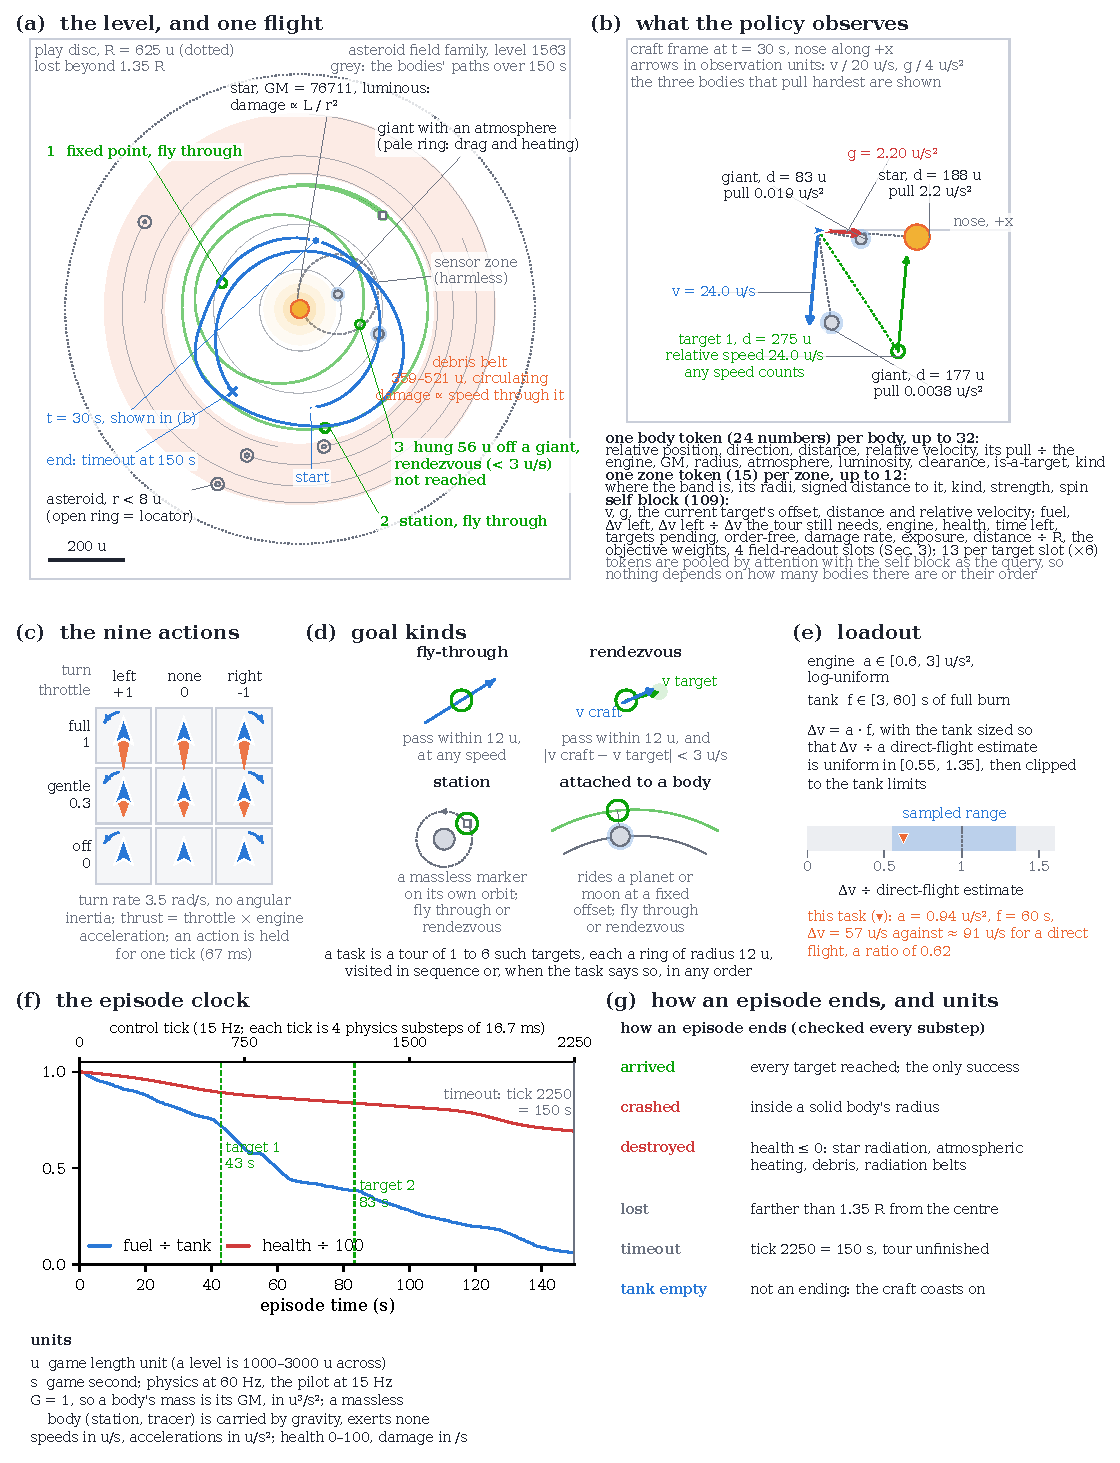
\includegraphics[width=\textwidth]{figures/task.pdf}
\caption{The task. (a) One level of the \code{asteroid\_field} family
(validation level 1563, radius 625\,u) with the bodies' paths over one
150\,s episode: a luminous star, two giants with atmospheres, a circulating
debris belt, asteroids drawn with locator rings since their true radius is
below 8\,u, and a three-target tour (a fixed flythrough, a station
flythrough, and a rendezvous hung 56\,u off the outer giant). The flight
shown is one of 32 sampled rollouts of a trained policy, all of which reach
the first two targets (at 43\,s and 83\,s) and then circle the star to the
clock without matching the giant's velocity; it is shown as the failure it
is. (b) What the policy observes at $t = 30$\,s, in the craft's frame: its
velocity and the local gravity, the three bodies that pull hardest, the
current target, and the contents of the body, zone and self tokens
(Appendix~\ref{app:obs}). (c) The nine discrete actions, turn $\times$
throttle. (d) The four goal kinds and their tolerances. (e) The loadout, with
the $\Delta v$ budget as a multiple of the direct-flight estimate and this
task's value marked. (f) Fuel and health of the flight in (a) against the
2250-tick clock, with the two arrivals marked. (g) The five ways an episode
ends, the one way it does not, and the units. Drawn by
\code{scripts/fig\_task.py}.}
\label{fig:task}
\end{figure}

\subsection{Three ways to picture the problem}
\label{sec:framings}

The rest of this paper returns repeatedly to three pictures of the task,
which are each correct and each suggest a different notion of difficulty,
and no one of which is sufficient alone.

The first is the plain reinforcement-learning loop, in which the craft
observes the field, acts, is rewarded for progress, and improves a policy by
gradient steps on that reward \cite{sutton2018,schulman2017}. An agent
trained this way does learn to fly (Section~\ref{sec:results}), but when the
craft enters a region in which nearby trajectories diverge exponentially, the
objective the policy gradient is climbing becomes rough at every scale below
the divergence length, and the gradient carries no usable descent direction
unless the algorithm's discount and control interval sit on the right side of
a threshold set by the field's Lyapunov exponent rather than by the algorithm
\cite{wang2023,metz2021,parmas2018}. Whether this environment's field crosses
that threshold is measured in Section~\ref{sec:chaos}.

The second picture treats the craft's flight as passage through a sequence
of regions of differing predictability, i.e. as a state machine whose states
are regimes rather than positions. In a well-behaved regime a trajectory can
be planned ahead with confidence, while inside a chaotic one the exit
trajectory cannot be predicted, by definition \cite{lorenz1963,grebogi1983},
but it can be bounded, i.e. the region can be entered in a way that constrains
the set of exits to something a plan on the far side can absorb, which is the
construction that reachable-set and tube-based formulations of control make
rigorous \cite{mitchell2005,mayne2005} and that belief-state planning gives a
probabilistic form \cite{kaelbling1998}. On this view a chaotic region is a
noise filter, and the navigator's plan is for what comes after it. This is
the picture closest to how mission designers reason about a close encounter,
and it is the one that makes difficulty depend on what lies after a region as
much as on the region itself.

The third picture is a stack of strategies, each adequate for a class of
levels and each subsumed by the next, in the sense that the options
framework gives to a hierarchy of behaviors \cite{sutton1999}. At the bottom
sits dead heading (point at the target and burn), adequate when gravity is
negligible against the engine; above it, leading a moving target; above that,
conic reasoning in which only the nearest massive body is accounted for and a
flight is a sequence of Keplerian arcs \cite{bate1971}; above that, the
deliberate use of encounters for assists \cite{flandro1966} and of the
field's own transport structure for low-energy transfers
\cite{belbruno1993,koon2000}; and at the top, models learned from experience
that make no such simplifying commitment. Each rung is a representation of
the field, and a level is hard on this picture when the rung a navigator
stands on is the wrong one for it. Of the three pictures, this is the one
that yields a closed-form difficulty measure, and it is developed in
Section~\ref{sec:eta}.

\FIG{the three pictures side by side: an observe-act-reward loop; a
trajectory entering and leaving a shaded region with a bounded exit cone; a
ladder of strategies from dead heading to learned model}

% =====================================================================
\section{Why a level of a given difficulty is hard to design}
\label{sec:hard}

A level generator that is asked for a hard level has to decide what hard
means, and the three pictures above make it clear that no single answer
exists \cite{furuta2021,dennis2020,rutherford2024}. A level can be hard for
at least six reasons: 1) the field is contested and a coarse representation
of it is wrong (the third picture); 2) an encounter scatters trajectories so
widely that nothing on the far side can be planned for (the second); 3) the
window in which a decisive action must be taken is narrower than a human
hand can hold; 4) the tank is short; 5) the hazards are dense; or 6) the
targets are placed so that one of these is unavoidable. A level that is hard
for one of these reasons may be trivial for every other, and the repair for
one does nothing for another, since widening a timing window does not change
a contested field and simplifying the field does not widen a window.
Interestingness, which is what a level designer ultimately wants, is related
to difficulty without being identical to it, since a level that is impossible
is not interesting and a level that is hard for an uninteresting reason (the
clock, as Section~\ref{sec:clock} argues) is merely frustrating. None of
these notions, moreover, can be checked by exhaustion.

\subsection{What it would take to check an answer}
\label{sec:complexity}

Consider the most naive possible procedure for establishing that a level is
solvable, which is to enumerate every control sequence and simulate each
one. The control at each of $T$ steps is a direction and a thrust magnitude,
both continuous, so even with a discretization to $a$ distinct actions per
step the number of sequences is $a^T$, and at $T = 2250$ this is beyond
reach for any $a > 1$; the discrete nine-action set used here does not
rescue the situation ($9^{2250}$ has more than two thousand digits), and the
underlying continuous problem has no finite enumeration at all. Formal
results in motion planning make the same point: the generalized mover's
problem is PSPACE-hard \cite{reif1979,hopcroft1984,canny1988}, and remains
so with moving obstacles even for a point robot of bounded velocity
\cite{reif1994}; finite-horizon planning under partial observation is
PSPACE-complete and its infinite-horizon form undecidable
\cite{papadimitriou1987,madani2003}; and reachability for quite simple
classes of continuous and hybrid dynamics is undecidable
\cite{moore1990,henzinger1998,blondel2000}. Note that these are results
about problem classes rather than about any single instance, and that
approximate search is not hopeless in principle, since kinodynamic planning
with bounded velocity and acceleration admits a polynomial-time
$\varepsilon$-approximation \cite{donald1993}; what they establish is that
no efficient general procedure exists, and that the field studied here,
which couples every body's position to the craft's acceleration at every
step, sits well inside the intractable regime.

Exhaustive checking is therefore replaced, in practice, by one of two
things, a simplifying assumption (a coarse model of the field, a restricted
family of control sequences, a short horizon) or a search that samples the
space and reports what it finds, and both are used in this paper. Both also
share a limitation that a chaotic regime makes acute. In a region where
nearby trajectories diverge exponentially, the numerical trajectory of a
given control sequence and the true trajectory of that sequence part company
within a few multiples of the Lyapunov time, since the shadowing of a
computed orbit by a true one breaks down in finite time when the local
expansion rate fluctuates \cite{hammel1987,sauer1997,sauer2002}, so that a
check which reports that a sequence arrives is a statement about a
trajectory the craft cannot actually fly, and the precision of the check
becomes the limit before its cost does. The same literature offers the
consolation on which this paper's method rests, which is that ensemble
statistics over many orbits remain reliable where individual orbits do not
\cite{boekholt2015,portegieszwart2018}. Thus, in general, a level's
difficulty cannot be read off from its definition and has to be measured
over a population, and the measurement is itself only as good as the probe
used to make it.

% =====================================================================
\section{Heuristics for difficulty and interestingness}
\label{sec:heuristics}

The quantities used in this paper to describe a level are heuristics, in the
sense that each is a cheap proxy for a property that cannot be computed
exactly, and the reader is asked to hold them as such. What follows is the
environment in enough detail to define them, then the quantities, then the
properties of the field that bear on whether they mean anything.

\subsection{The environment}
\label{sec:env}

The simulation is planar with gravitational constant $G = 1$, so each body's
mass is a gravitational parameter $GM$; lengths are in game units (u) and
times in game seconds (s), with a typical level spanning 1000--3000\,u.
Bodies attract one another and are advanced by a kick-drift-kick leapfrog
integrator at a 1/60\,s substep, i.e. by the symplectic family standard in
n-body work \cite{wisdom1991,rein2015}, with the field inside a body's
radius falling off linearly (as for a uniform sphere) so that accelerations
are finite everywhere. The craft is a test particle (it is accelerated by
every body and accelerates none), so a level's body trajectories are
determined by the initial snapshot, which is what allows a level to be
reproduced from a seed, replayed exactly, and integrated independently by a
browser client from a snapshot of about 1.5\,KB. Four physics substeps make
one control tick, so the craft and a human player both act at 15\,Hz.

A task instance is a short tour of between one and six targets, each either
a point in free space, a station, or a point carried by a moving body at a
constant offset, with an arrival radius (12\,u) and a velocity tolerance
(any speed for a flythrough target; within 3\,u/s of the target's own
velocity for a rendezvous, which is materially harder and is drawn only for
a target that moves), in a fixed or a free order. The craft carries a tank expressed as
seconds of full-throttle burn and an engine acceleration, both drawn per
instance from ranges chosen so that no craft can ignore gravity and fly
straight at its target. Hazards are radiation from luminous bodies,
atmospheric heating, debris fields and radiation belts. An episode ends on
arrival at the last target, collision, destruction by accumulated damage,
departure past 1.35 times the level radius, or the clock; an empty tank is
not an ending, since the craft coasts on and the episode runs to the clock,
which is one of the reasons the clock matters as much as it does
(Section~\ref{sec:clock}). Appendices~\ref{app:obs}
and~\ref{app:goals} give the observation vector and the goal conditions in
full.

Levels are generated in twelve families, each of which exists to produce a
distinct regime of the field, and they are listed in Table~\ref{tab:families}
with the reason each is in the set. Three (\code{sol\_like}, \code{jovian},
\code{saturnian}) are hierarchical systems in which one body dominates almost
everywhere, so that a coarse one-body representation is nearly always
adequate; three (\code{binary\_star}, \code{trinary}, \code{star\_cluster})
are systems of comparable masses in which no single body dominates anywhere;
and the remainder each introduce one specific feature, i.e. dense small
bodies (\code{asteroid\_field}), a tightly packed system
(\code{compact\_system}), extended hazard zones (\code{debris\_maze}), a very
massive compact object (\code{bh\_cluster}), intense radiation
(\code{pulsar}), and a single unbound body passing through
(\code{rogue\_flyby}). Generating levels procedurally across families, rather
than training and testing on a fixed set, is the standard means of measuring
whether a policy has learned a task or a level
\cite{cobbe2019,cobbe2020,justesen2018}. A generated level is accepted only
if it remains well-behaved (no collisions, no ejections, bounded energy
drift) for a validation horizon, and accepted levels are stored as snapshots
at 20\,s intervals so that an episode may begin at any of several epochs.
Four pools are used throughout: 18,000 training levels, 2,700 validation
levels from the same families, and 1,200 holdout levels from families never
trained on, each validated to 300\,s (twice an episode) and carrying eight
snapshots; and 1,800 long-horizon levels validated to 900\,s and carrying
sixteen snapshots, for experiments at extended clocks
(Section~\ref{sec:clock}).

\begin{table}[t]
\centering
\footnotesize
\begin{tabular}{llp{4.8cm}r}
\toprule
Family & Regime & Why it is in the set & Median $\eta$ \\
\midrule
\code{sol\_like}        & hierarchical & one star, well-separated planets; the baseline in which a coarse model is right almost everywhere & 0.0027 \\
\code{jovian}           & hierarchical & a giant with a retinue of moons; dominance passes between bodies within a small region & 0.0080 \\
\code{saturnian}        & hierarchical & as \code{jovian}, with a ring system that adds a hazard band & 0.0058 \\
\code{compact\_system}  & hierarchical & many bodies packed close; short orbital periods relative to the episode & 0.0017 \\
\code{asteroid\_field}  & hierarchical & many small bodies; collision risk without a change in the dominant field & 0.0013 \\
\code{debris\_maze}     & hierarchical & extended debris zones; the hazard, not the gravity, shapes the route & 0.0005 \\
\code{bh\_cluster}      & intermediate & a compact massive object among lighter bodies; a steep field with a contested shell & 0.068 \\
\code{binary\_star}     & contested & two comparable masses; no point at which one body dominates & 0.35 \\
\code{trinary}          & contested & three comparable masses & 0.47$^{\dagger}$ \\
\code{star\_cluster}    & contested & several comparable masses; contested everywhere & 0.53 \\
\code{pulsar}           & hierarchical & a luminous body whose radiation, not its gravity, is the constraint & 0.0026$^{\dagger}$ \\
\code{rogue\_flyby}     & transient & one unbound body crossing the level; the dominant field changes during the episode & 0.061$^{\dagger}$ \\
\bottomrule
\end{tabular}
\caption{The twelve level families. Median $\eta$ (the fraction of local
gravity a one-body model discards, Section~\ref{sec:eta}) over the playable
area of each family's levels, computed by \code{scripts/paper\_figures.py}
from the long-horizon pool. $^{\dagger}$The three holdout families are
absent from that pool and were measured on the holdout pool at its first
snapshot ($n = 30$ levels each); \code{rogue\_flyby} is transient, with the
unbound body 1300--1600\,u out at that epoch, so its $\eta$ at later epochs
is higher.}
\label{tab:families}
\end{table}

\subsection{Nontrivial difficulty}
\label{sec:eta}

The representation a person brings to a gravitational field is almost always
the one-body representation, in which the dominant attractor is identified,
its field is taken for the whole field, and trajectories are reasoned about
as conic sections. This is instantiated in the environment by a function,
\code{gravity\_at(topk=k)}, that restricts the craft's felt gravity to the
$k$ strongest attractors at its current position and discards the rest, with
$k = 1$ being patched conics and $k = 0$ the truth; bodies always move
truthfully, and only the test particle's felt force is restricted, so that a
plan made inside the coarse representation can be flown in the true field
and the discrepancy observed.

With $a_{\mathrm{full}}$ the true local acceleration and $a_{\mathrm{dom}}$
the acceleration due to the single strongest body, the fraction of the field
that a one-body representation throws away is
\begin{equation}
\eta \;=\; \frac{\lVert a_{\mathrm{full}} - a_{\mathrm{dom}} \rVert}
{\lVert a_{\mathrm{full}} \rVert},
\end{equation}
which is near zero where patched conics is adequate and near one where it is
not. However, $\eta$ alone is not difficulty, because a craft with a large
enough engine can absorb the error. With $\Delta v_{\mathrm{tank}}$ the tank
expressed as a velocity budget, $\lVert g \rVert$ the local gravitational
acceleration and $T$ the remaining flight time, the authority
\begin{equation}
A \;=\; \frac{\Delta v_{\mathrm{tank}}}{\lVert g\rVert\, T}
\end{equation}
is the tank in units of the impulse gravity itself will deliver over the
flight ($A > 1$ meaning the craft can out-push the field, $A < 1$ that it
cannot), and the quantity used to score a level is their ratio,
\begin{equation}
\dd \;=\; \frac{\eta}{A},
\end{equation}
which has the direct reading of the share of the tank that flying the wrong
representation would cost. Both ingredients are available in closed form from
the level snapshot and the task specification, so $\dd$ requires no
simulation and thousands of candidate levels can be scored for free, with
expensive planning reserved for levels already known to sit where they are
wanted. Moreover, it inverts: solving for the tank gives
$\Delta v_{\mathrm{tank}} = \eta \lVert g \rVert T / \dd$, so that a level
can be placed on a chosen rung by solving for the tank (fuel is only ever
added when retuning, since a level starved onto a high rung is infeasible
rather than demanding).

An ordinary level in this environment sits at $\dd \approx 0.0014$, with
$\eta = 0.0036$ and $A = 3.8$, which is to say that gravity supplies about a
quarter of the tank's worth of impulse over a flight but a single body
explains 99.6\% of the field, so that patched conics is adequate on an
ordinary level and $\eta$ has to be raised by construction. That $\dd$
measures what it is meant to was checked by comparing a planner restricted
to the one-body representation against one with the true field on levels
pooled by $\dd$ band (24 levels per band, two bands): below $\dd = 0.1$ the
two were indistinguishable (32\% versus 42\% arrival, Fisher's exact
$p = 0.74$), while above it they separated (13\% versus 54\%, $p = 0.005$),
with the coarse planner failing every level on the top rung. Note that the
per-rung figures within those bands, at $n = 8$, are not individually
significant, and only the pooled comparison should be read.

Where in a level a coarse representation breaks is governed by instantaneous
force competition rather than by the field's resonance structure, although
the latter is the natural candidate from the literature on constructed chaos
\cite{chirikov1979,wisdom1980,deck2013}, since resonance overlap describes
what happens over many orbital periods while an episode here is a fraction
of one, and placing targets in the Wisdom band raises $\eta$ only from
$0.0026$ to $0.0172$, sixfold and still negligible, because a few Hill
radii from a secondary has $\eta \approx 0.02$ throughout. The relevant
surface for an episode this short is the one on which a secondary's pull
equals its primary's, at a distance $d = a\sqrt{m/M}$ from a secondary of
mass $m$ orbiting a primary of mass $M$ at semi-major axis $a$ (about half a
Hill radius, and distinct from the Laplace sphere of influence used in
patched-conic design \cite{bate1971}). Figure~\ref{fig:eta}(a) shows $\eta$
measured on shells around the second-most-massive body of 297 levels
spanning nine families, as a median over 24 directions at each radius: it
rises from $0.09$ at $0.3\times$ the equal-pull radius to a peak of $0.43$
at $1.0\times$ and falls to $0.24$, $0.066$ and $0.020$ at $2\times$,
$4\times$ and $8\times$. The peak value depends strongly on how it is
sampled, since along the line joining primary and secondary the two pulls
oppose and $\eta$ exceeds one; the angular median is the conservative
statistic and the one the level generator is tuned against, with target
placement in contested levels confined to the $0.8$--$1.3\times$ shell. The
larger lever by far is family choice (Figure~\ref{fig:eta}(b)): median $\eta$
over the playable area spans three orders of magnitude from
\code{debris\_maze} ($0.0005$) to \code{star\_cluster} ($0.53$), so that
systems of comparable masses are contested everywhere and hierarchical
systems only within thin shells that must be aimed at deliberately.

\begin{figure}[t]
\centering
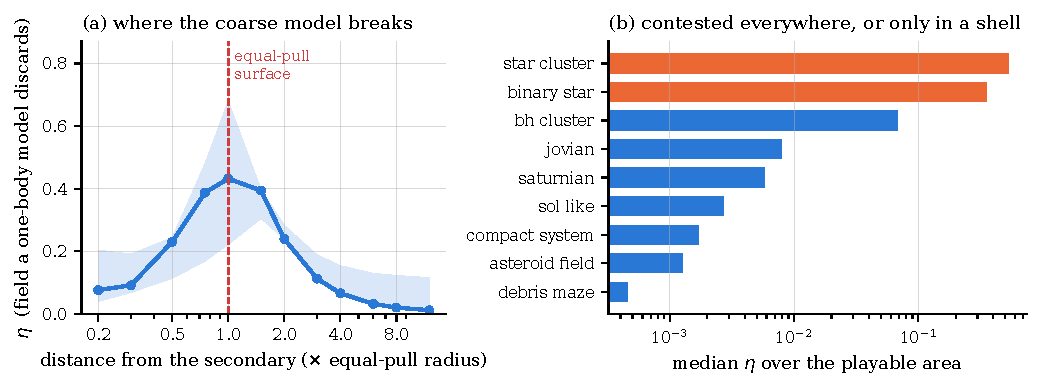
\includegraphics[width=\textwidth]{figures/eta.pdf}
\caption{(a) The fraction $\eta$ of local gravity that a one-body
representation discards, against distance from a secondary in units of the
equal-pull radius $a\sqrt{m/M}$; median over 24 directions on each shell,
across 297 levels from nine families, with the interquartile range shaded.
(b) Median $\eta$ over the playable area by family, with the two families
that are contested everywhere in orange. Computed by
\code{scripts/paper\_figures.py}.}
\label{fig:eta}
\end{figure}

Figure~\ref{fig:phase} makes these quantities visible on four real levels,
one per family (chosen as the level whose median $\eta$ is nearest its
family's median, so that none was chosen on its appearance), as fields over
the playable area: $\eta$; a finite-time Lyapunov exponent over 20\,s,
measured by displacing a coasting particle and integrating the separation
against the true ephemeris; and the single-burn outcome map, which records,
for the level's start, which burn headings and burn times reach the target.
The $\eta$ row separates the families at a glance, since a hierarchical
level is dark everywhere except in thin rings around its planets while a
contested level is bright everywhere and the equal-pull surface is a real
dividing curve through the middle of it. The outcome row does not separate
them, and the reason is instructive: a single-burn decision space is shaped
by the task (the start orbit, the target's motion, the authority $A$) at
least as much as by the family, so that the star cluster shown has a clean
diagonal winning stripe (the signature of leading a moving target, since
the right heading advances with the burn time) and the binary star a
single narrow band, while two other levels from the same families would
show different shapes. A claim about the decision space of a family, as
opposed to a task, needs many tasks per family and is not made here.

\begin{figure}[p]
\centering
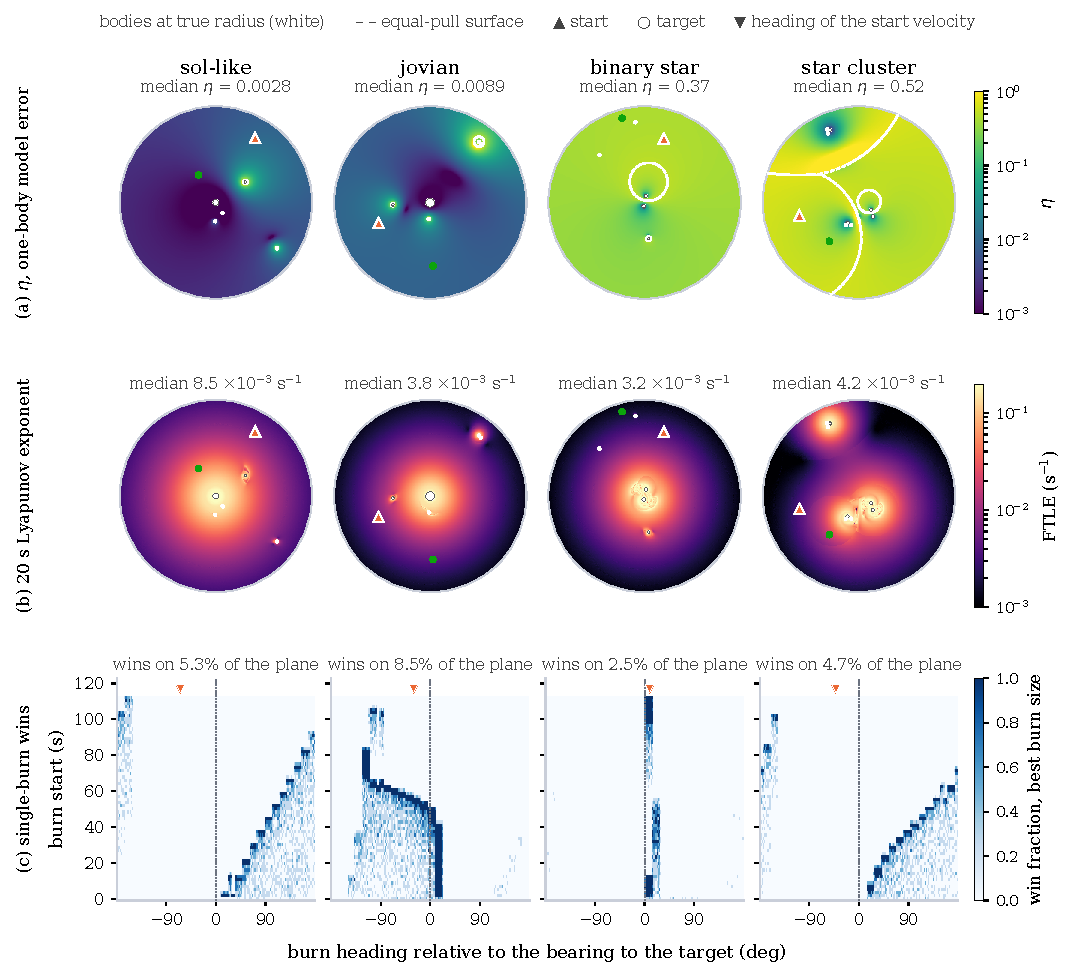
\includegraphics[width=\textwidth]{figures/phase.pdf}
\caption{Computed portraits of four levels, one per family, with families
as columns. (a) The $\eta$ field over the playable area on a logarithmic
scale, with bodies at true radius and the measured dominance boundary (where
the strongest attractor changes) dashed; the start and target are marked. (b)
A 20\,s finite-time Lyapunov exponent from a displaced coasting particle,
integrated against the true ephemeris. (c) The single-burn outcome map for
the level's own task: the fraction of jittered draws that arrive, over burn
start and burn heading relative to the bearing to the target, taking the
best of four burn sizes. One color scale per row. Row (c) is the decision
space of one task, not a property of the family. Computed by
\code{scripts/fig\_phase.py} on 368,640 full-episode rollouts per level.}
\label{fig:phase}
\end{figure}

\subsection{Trivial difficulty}
\label{sec:trivial}

Separate from whether a representation suffices is whether a correct plan
can be executed, i.e. whether the window in which a decisive action must be
taken is wide enough for the hand that must take it. Measured human limits
(roughly 20\,ms of motor onset jitter for a practiced discrete action
\cite{repp2005}, 200--250\,ms of simple visual reaction time
\cite{woods2015}, and visuomotor feedback responses beginning 120--180\,ms
after a perturbation with a closed-loop correction ceiling near 3\,Hz
\cite{franklin2011,franklin2014}) give the scale, and the 66.7\,ms control
tick, already coarser than a trained hand, makes the comparison generous.
Every level is banded on this axis as well as on $\dd$, and the two are
never combined (Section~\ref{sec:hard}). This kind of difficulty is called
trivial here because it says nothing about the field, and it is not treated
further.

\subsection{Chaos on episode timescales}
\label{sec:chaos}

Several of the pictures in Section~\ref{sec:framings} presuppose that the
field is chaotic on the timescale of an episode, and the threshold at which
chaos matters to a learner is sharp enough that the field has to be checked
against it. Wang, Herbert and Gao \cite{wang2023} show that the
reinforcement-learning objective is $\alpha$-H\"older with
$\alpha = \log(1/\gamma)/\lambda$ for a system with maximal Lyapunov
exponent $\lambda$ and discount $\gamma$, becoming fractal, and losing any
usable descent direction, when $\lambda$ exceeds $\log(1/\gamma)/\Delta t$;
at the discount of $\gamma = 0.999$ and the $1/15$\,s control interval used
here that threshold is $\lambda_{\mathrm{crit}} = 0.0150\,\mathrm{s}^{-1}$,
corresponding to a Lyapunov time of 67\,s. The measured predictability
horizon of the environment (the time at which one control tick's worth of
thrust error grows past the 12\,u arrival tolerance) is 52--74\,s across
eight families, close enough to that figure that bounding the exponent is
not sufficient and it has to be measured.

The divergence is ballistic, since $d\ln(\mathrm{sep})/dt$, which falls as
$1/t$ for linear growth and stays flat for exponential growth
\cite{benettin1980,ott2002}, decays in the measured separations in the
manner of linear growth: pure linear growth predicts a 150\,s-to-75\,s slope
ratio of exactly $0.50$, and the measured ratio is $0.33$--$0.64$ with a
median near $0.56$ (16 levels in each of eight families, one tick of thrust
as the perturbation). Fitting $\mathrm{sep} = a\,t\,e^{\lambda t}$ to divide
out the ballistic factor gives $\lambda = 0.0045$--$0.0086\,\mathrm{s}^{-1}$
(90th percentile near $0.010$), roughly a factor of two below
$\lambda_{\mathrm{crit}}$, with only the tail of \code{star\_cluster}
exceeding it. A Lyapunov time of about 140\,s against a 150\,s episode is one
e-folding per episode, or about 2000 control steps per e-folding, whereas
the reinforcement-learning results on chaotic systems in the literature sit
at 10--100 steps per e-folding \cite{bucci2019,rabault2019,vignon2023}, and
the classical chaos-control results treat that sensitivity as the thing that
makes small control effective \cite{ott1990,shinbrot1990}; the environment
is well inside the benign regime. The uncertainty exponent of the arrival
basin \cite{grebogi1983,mcdonald1985,aguirre2009}, which is near one for a
smooth boundary and near zero for a fractal one, measures $0.53$--$1.02$
once enough perturbation samples are used to fit it (768 per level; with 96
the flip counts are small integers and no exponent can be trusted),
consistent with the Lyapunov result. Thus, the field is quasi-integrable on
the timescale of an episode, in the sense in which a near-integrable
Hamiltonian system retains most of its invariant tori under perturbation and
drifts only over times exponentially longer than its orbital period
\cite{kolmogorov1954,arnold1963,nekhoroshev1977}, and in the same sense in
which the solar system is chaotic with a Lyapunov time of millions of orbits
\cite{laskar1989,sussman1992}, and where chaos is wanted, as it is for the
second picture of Section~\ref{sec:framings}, it has to be built into a
level, chiefly by episodes long relative to orbital periods (closer
encounters and tighter binaries help less).

\subsection{Solvability}
\label{sec:solvable}

A closed-form $\dd$ says how much a wrong representation would cost but not
whether a level can be flown at all, and for that there is no substitute for
attempting it with the strongest navigator available. Here that is a
cross-entropy-method trajectory optimizer \cite{rubinstein1999}, of the
sampling-based kind that runs well on a graphics processor
\cite{williams2017}: piecewise-constant control segments over the episode
(48 segments of 3.1\,s at the 150\,s clock), seeded from a scripted reflex
controller and from an explicit zero-thrust candidate, iteratively refined
toward an arrival objective over 96 samples and 7 iterations, with the
zero-thrust seed included because throttle is parameterized through a
sigmoid and an all-coast plan is otherwise never drawn, which caused the
optimizer to fail on the levels where coasting is optimal. A level is called
solvable if the optimizer arrives or if any member of an enumerated one- or
two-burn family of control sequences arrives, and a level that nothing can
fly receives no difficulty label; this is a design decision, not a result,
and it is the nearest relative in this paper of the observation that
levels an agent always or never solves carry no curriculum information
\cite{rutherford2024,dennis2020}.

Two properties of this yardstick bear on every use of it. Firstly, its
failure is weak evidence, since a given optimizer configuration flies a given
level or does not, and a run of failures over a small set of levels is
consistent with a true success rate well above zero (zero successes in
twelve attempts is consistent with a rate of 16\%, the rate observed on the
same level family at $n = 32$, at probability $0.13$), so that a level class
should be called infeasible only on a sample sized to the claim
\cite{agarwal2021,colas2018}. Secondly, and more fundamentally, the true
optimum for a level is never in hand, because the optimizer is a sampled
search over a restricted control family on a problem that
Section~\ref{sec:complexity} argues cannot be solved exhaustively, so that
every difficulty label in this paper is relative to a navigator that is
itself imperfect in ways that cannot be fully characterized, and a level
labelled unflyable is one that nothing tried could fly. More computation
does not remove this limitation, which is the condition of the problem, and
it is why the paper treats a learning agent (Section~\ref{sec:learning}) as
a second, independent probe of the same levels as well as the thing being
graded.

\subsection{The episode clock}
\label{sec:clock}

Of the constraints a level places on a craft (time, fuel, and exposure to
damage), time is the least interesting, and it is also the one most easily
mistaken for difficulty. This is a position, not a finding, since deadlines
and launch windows are real constraints in every mission-design source cited
above, but it is the position the measurement below supports.
Fuel is a harder constraint, because it is consumed and cannot be recovered,
and exposure is the most interesting, because radiation, debris and
atmosphere each have their own geometry and dynamics and because avoiding
them shapes a route in ways the gravity alone would not. The clock, by
contrast, mostly penalizes a craft that chooses an energy-efficient path over
a fast one, which is the choice every mission in Section~\ref{sec:field} was
praised for making.

The evidence that the 150\,s clock of this environment is binding in that
way comes from the optimizer of Section~\ref{sec:solvable} flown on 32
two-target levels at four clocks, with control resolution held at 3.1\,s per
segment so that a longer clock buys more segments rather than coarser ones
(Figure~\ref{fig:clock}). Arrivals rise from $5/32$ at 150\,s to $8/32$ at
300\,s and $13/32$ at 600\,s, then fall back to $11/32$ at 900\,s; timeouts
fall monotonically from 18 to 5; and crashes, destructions and fuel
exhaustions go from 9 at the shortest clock to 16 at the longest, though not
monotonically, so that of the thirteen timeouts a longer clock removes,
about half become arrivals and half become hazard endings. Thus, for the
optimizer at 150\,s, a substantial fraction of what the environment scores
as failure is the clock, and the useful ceiling for this task class is near
600\,s, beyond which hazard exposure is the binding constraint.

The same experiment on a weaker navigator gives the opposite reading, and
the contrast is the point. Evaluation suites were rebuilt from a
900\,s-validated pool at a 600\,s clock (same families and task
specifications as the 150\,s suites, different levels, so same-family rather
than paired), and the scripted reflex pilot was flown on them: its arrivals
after the 150\,s mark are 1/480, 3/197, 1/47 and 0/136 on the easy, medium,
hard and blind suites, and its 150\,s timeouts (102, 146 and 147 of about
600 on the medium, hard and blind suites) became fuel exhaustions and
collisions at 600\,s rather than arrivals (medium suite: timeouts 102 to 17,
fuel exhaustions 53 to 105, arrivals 206 to 197). A longer clock, that is,
gives a navigator the time to finish a path it could not otherwise finish,
or the time to exhaust its tank and fall into a body, and which of the two
it gets depends on the navigator and not on the clock.

The learned policy, trained at a 600\,s clock, is a third case, and the one
that argues most strongly against treating the clock as a free parameter.
Three seeds of the best 150\,s configuration were trained for 3000 updates
with the clock at 600\,s on the long-horizon pool and evaluated on the 600\,s
suites (same families and task specifications as the 150\,s suites, different
levels, so same-family rather than paired; and the blind suite is not blind
at this clock, since no long-horizon pool carries the holdout families). Two
seeds learned and one did not: the two that learned reached 68\% and 74\% on
the easy suite and 26\% and 32\% on the medium suite, against 90\% and 42\%
for the same configuration at 150\,s, while the third never exceeded 19\% on
the easy suite and finished at 4\%, so that the mean over seeds is
$48.9 \pm 38.6$, $19.8 \pm 16.1$, $3.9 \pm 3.6$ and $13.1 \pm 10.5$ on the
four tiers. Note that the dominant ending for the policies that did learn
was still the clock: 37--42\% of medium-suite tasks timed out at 600\,s,
against roughly a third at 150\,s, so that four times the time produced
more timeouts, not fewer. The explanation this paper can offer, without
having tested it, is the discount: $\gamma = 0.999$ gives the value estimate
a horizon of about 65\,s at 15\,Hz, which is a reasonable fraction of a
150\,s episode and a ninth of a 600\,s one, so that a policy trained at the
longer clock is rewarded for progress it cannot see the end of and has every
reason to drift. Whether raising the discount to match the clock recovers
the 150\,s performance is \MEASURE{queued: $\gamma = 0.9995$ and $0.9998$
(about 130\,s and 330\,s of lookahead) at 600\,s, three seeds each}; what
can be said now is that a longer clock is not a free parameter for a learner
either, and that the sense in which 150\,s was arbitrary (Section
\ref{sec:discussion}) does not make 600\,s correct.

There is a reason the clock cannot simply be set long enough to settle the
question, and it is worth stating because it bears on what solvability
means. Consider a navigator that does nothing at all. The craft is a test
particle in a bounded gravitational system, and a bounded Hamiltonian system
is recurrent, in the sense Poincar\'e established for exactly this problem
\cite{poincare1890}: almost every trajectory returns arbitrarily close to
its starting state, and so, given enough time, a coasting craft will pass
within the arrival radius of any target it can reach at all, unless an
invariant surface of the kind that survives perturbation in a near-integrable
system \cite{kolmogorov1954,arnold1963} happens to separate it from that
target permanently. Thus, for a flythrough tour, the zero-action policy
succeeds with probability approaching one as the clock lengthens, and the
only stopping criterion that is not a choice is divergence, i.e. the craft
leaving the system; inside it, there is always an improbable path that has
not yet been given time to occur (in the limit of a system collapsing
gravitationally to a point, every path is that path). A finite clock is
therefore a definition rather than a measurement of the task, and
solvability is relative to a time budget in the same way that
Section~\ref{sec:eta} makes it relative to a fuel budget, and the question
becomes how much a given navigator's success depends on the allowance. The
same fact is what makes the exhaustive check of Section~\ref{sec:complexity}
ill-posed even in principle, since without a horizon the question of whether
a control sequence has failed has no finite answer for a sequence that stays
in the system.

The zero-action navigator was therefore measured directly
(Figure~\ref{fig:noop}). Coasting from the start of every task in the 600\,s
suites for 900\,s (13,500 ticks, the levels' validated horizon), the fraction
of tasks in which the craft passes within the arrival radius of any target
(velocity tolerance and tour order ignored) is 2.3\%, 2.9\%, 5.1\% and 3.7\%
at 150\,s on the easy, medium, hard and blind suites, and 5.3\%, 6.6\%, 9.8\%
and 6.9\% at 900\,s, still rising at the end at about 0.2--0.5 percentage
points per 100\,s; strict completion of the tour as specified by coasting is
0--1.2\% on every tier except easy (5.3\%, where contact is completion). Over
the same interval the fraction of tasks ending in collision, destruction or
escape rises at about 2.5 points per 100\,s on the three harder tiers, to
26--27\% at 900\,s. To see where the contact curve goes, a pool of 900 levels
was validated to 9{,}000\,s (ten episodes; 80--100\% of generated levels
survive that long, so bounded systems from these generators stay bounded)
and the same measurement run on it: contact reaches 8.7\%, 9.8\%, 12.9\% and
11.8\% by 9{,}000\,s and is flat over the last 300\,s, because the craft is
dead, with 78--80\% of the non-easy tasks ended by then and destruction by
accumulated damage the commonest ending. Thus, patience alone buys a
coasting craft three to five points of contact between 150\,s and 900\,s and
another three to six between 900\,s and 9{,}000\,s, and the race between
the improbable path and exposure is won by exposure; in this environment the
stopping criterion that recurrence fails to supply is supplied instead by
the hazards, and the constraint the author ranks most interesting is also
the one that bounds the clock.

\begin{figure}[t]
\centering
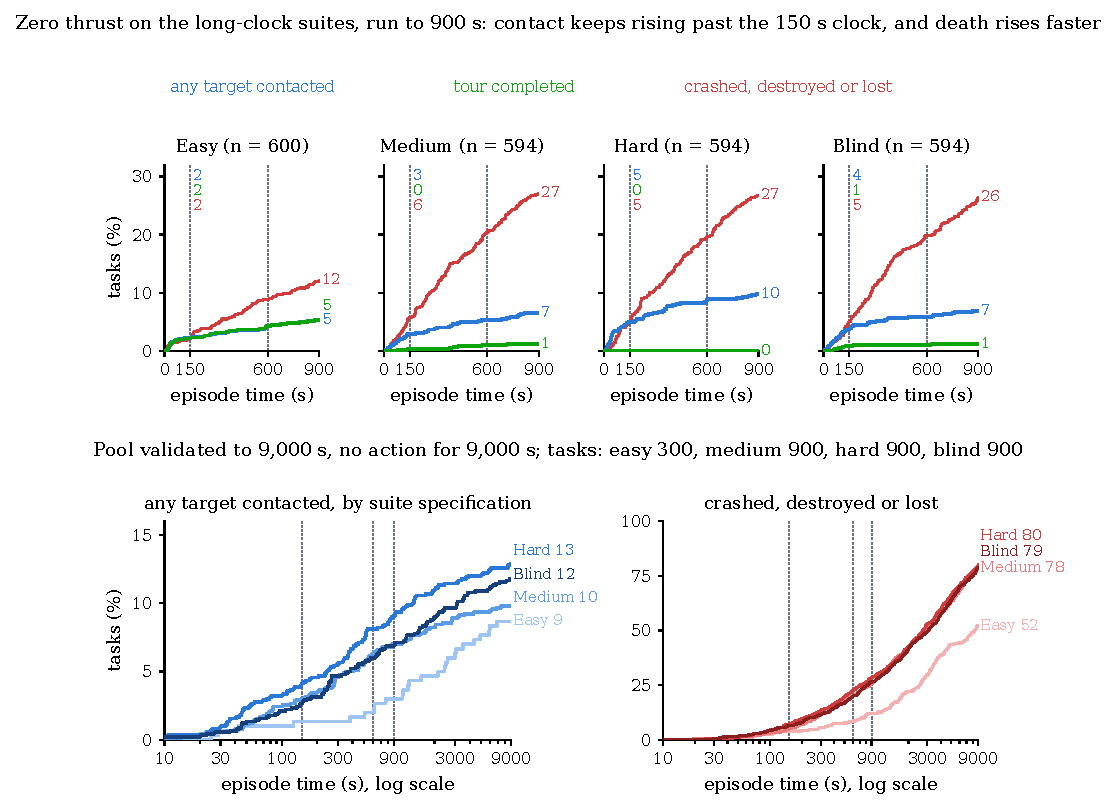
\includegraphics[width=\textwidth]{figures/noop.pdf}
\caption{A craft that never thrusts. Top: on the four 600\,s suites run to
900\,s, the cumulative fraction of tasks in which the craft has passed
within the arrival radius of any target, completed the tour as specified,
or ended in collision, destruction or escape, with rules at the 150\,s clock
and at 600\,s and the values at 150 and 900\,s marked. Bottom: on 900 levels
validated to 9{,}000\,s, the same contact and death curves on a logarithmic
time axis, by suite specification. Computed by \code{scripts/noop\_clock.py};
the two rows are same-specification, not paired.}
\label{fig:noop}
\end{figure}

\begin{figure}[t]
\centering
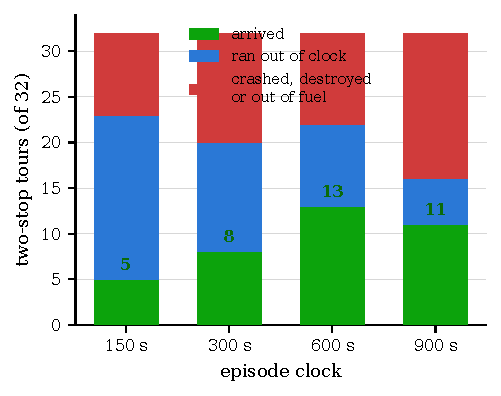
\includegraphics[width=0.46\textwidth]{figures/clock.pdf}
\caption{Thirty-two two-target levels flown by the reference optimizer at
four episode clocks, control resolution held at 3.1\,s per segment. Timeouts
fall monotonically, arrivals peak near 600\,s, and hazard endings rise.}
\label{fig:clock}
\end{figure}

% =====================================================================
\section{The learning agent}
\label{sec:learning}

A trained agent is used here both as a subject, evaluated on the levels as
any agent would be, and as an instrument, since where and how it fails is a
measurement of the levels that no closed-form quantity provides. The second
use is the more important one for the argument, and it requires that the
training procedure be ordinary enough that its failures are attributable to
the levels rather than to the procedure.

The policy is an actor-critic over the ego-centric observation of
Appendix~\ref{app:obs}: a fixed self block, one token per body and one per
hazard zone, with the tokens embedded and pooled two ways (multi-head
cross-attention with the craft's own features as the query, and a masked
max-pool), so that nothing depends on the number or order of bodies and the
same weights run on any level. The network has an embedding width of 128,
four attention heads and 285,322 parameters, which is small by the standard
of current general-purpose agents \cite{lee2025}. Training uses proximal
policy optimization \cite{schulman2017} with generalized advantage
estimation \cite{schulman2016} in a fully vectorized loop of the kind that
accelerator-native physics environments make practical \cite{matthews2025}
(1024 parallel environments by 128 steps, i.e. 131,072 transitions per
update; four epochs of eight minibatches; learning rate $3 \times 10^{-4}$
annealed linearly to a tenth; $\gamma = 0.999$; $\lambda = 0.95$; clip
$0.2$; entropy coefficient annealed from $0.01$ to $0.002$; value
coefficient $0.5$; gradient norm clipped at $0.5$), for 3000 updates or 393
million environment steps per run, which on the hardware used takes about
67 minutes. A curriculum \cite{bengio2009,narvekar2020} ramps the share of
rendezvous targets ($0.1 \to 0.45$), the maximum tour length ($1 \to 3$)
and, after the craft can fly at all, the share of levels whose targets are
placed in the contested equal-pull shell ($0 \to 0.35$), while the tank and
engine start generous and tighten to their full ranges.

Evaluation is on four frozen suites of about 600 task instances each,
described in Table~\ref{tab:suites} and held fixed across every run, with a
scripted reflex controller (proportional navigation with gravity
compensation, hereafter the reference pilot) scored on the identical
instances as a yardstick. Six hundred instances give roughly two percentage
points of binomial noise on a suite success rate, which is small against the
differences reported below; the larger source of variance is the training
seed, and every comparison between configurations is therefore made on seed
means over five independent runs per configuration, following the
statistical practice recommended for deep reinforcement learning
\cite{agarwal2021,henderson2018,colas2018}.

\begin{table}[t]
\centering
\small
\begin{tabular}{llcccccr}
\toprule
Suite & Pool & Targets & Rendezvous & Budget & Families & $n$ & Pilot \\
\midrule
easy   & validation & 1   & none      & $1.0$--$1.5\times$  & 3 hierarchical & 600 & 85.3\% \\
medium & validation & 1--2 & 25\%     & $0.8$--$1.25\times$ & all trained    & 594 & 34.7\% \\
hard   & validation & 2--3 & 50\%     & $0.7$--$1.05\times$ & all trained    & 594 & 7.6\% \\
blind  & holdout    & 1--3 & 35\%     & $0.75$--$1.15\times$ & never trained & 600 & 31.8\% \\
\bottomrule
\end{tabular}
\caption{The evaluation suites. Budget is the tank as a multiple of the
direct-flight $\Delta v$ estimate; the hard suite's budget is usually
insufficient for a direct flight, so that gravity must do some of the work.
Rendezvous is the probability that a target is a rendezvous given that it
moves (a station or a target carried by a body, drawn with probability
0.45--0.6 per target), so the unconditional share is roughly half the column.
The blind suite's tours are order-free 30\% of the time. Pilot is the
reference pilot's success rate on the identical instances.}
\label{tab:suites}
\end{table}

% =====================================================================
\section{Results}
\label{sec:results}

\subsection{Performance against the reference pilot}

Table~\ref{tab:main} gives the final success rate of the best configuration
found (the policy told $\eta$ and the stretching rate, for reasons given
below), as the mean of each run's last three checkpoints over five seeds,
against the reference pilot on the same instances. The learned policy
exceeds the pilot on the three suites drawn from trained families, by 3.5 to
7.2 percentage points, and falls 2.6 points short of it on the holdout suite,
which is the only suite in which the policy sees level families it was never
trained on and the only one in which the tour order is sometimes the
navigator's to choose. Note that the reference pilot is a weaker yardstick
than its rates suggest, since on a comfortable-tank instance set it arrives
63.3\% of the time and its dominant failure is collision (21.6\% of
instances) rather than fuel exhaustion (4.7\%) or timeout (7.8\%), so that
every margin quoted against it is softened by an opponent that flies into
bodies one time in five, though the absolute rates are unaffected.

\begin{table}[t]
\centering
\small
\begin{tabular}{lrrrr}
\toprule
& Easy & Medium & Hard & Blind \\
\midrule
Learned policy (5 seeds) & $90.4 \pm 1.8$ & $41.9 \pm 2.3$ & $11.1 \pm 1.0$ & $29.2 \pm 1.2$ \\
Reference pilot          & $85.3$ & $34.7$ & $7.6$ & $31.8$ \\
\midrule
Difference               & $+5.1$ & $+7.2$ & $+3.5$ & $-2.6$ \\
\bottomrule
\end{tabular}
\caption{Percentage of task instances completed, mean $\pm$ standard
deviation over five training seeds for the policy told $\eta$ and the
stretching rate (the \code{eta,stretch} configuration), against the
reference pilot on the identical instances. \TODO{the first draft's table
used the no-channel arm (89.4/41.7/10.7/30.2); this uses eta,stretch, which
is now the default; confirm which the author prefers as "the" result}}
\label{tab:main}
\end{table}

\subsection{Training budget}
\label{sec:budget}

Every configuration compared in this paper was trained for 3000 updates
(393 million environment steps), and the question of whether that budget is
where the comparisons should be made was answered by training the best
configuration for 10,000 updates (1.31 billion steps, about 3.5 hours per
run on the hardware used) at two seeds. The gain is large on every tier
(Table~\ref{tab:budget}): $+4.7$, $+15.3$, $+7.8$ and $+11.7$ percentage
points over the five-seed 3000-update mean on the easy, medium, hard and
blind suites, with seed standard deviations of $0.1$--$2.5$ points, and the
medium-suite curve of the longer runs rises from $47.8\%$ at update 3000
through $52.4\%$ at 6000 to $57.7\%$ at 10,000 without flattening. Thus, the
agent of Section~\ref{sec:learning} is under-trained at 3000 updates by a
margin larger than most of the effects reported in this paper, and the
ablations of Section~\ref{sec:instruments}, which were run at that budget,
are comparisons between under-trained policies; the direction of an effect
measured there is likely to survive more training, as the budget runs show
the same ordering across tiers, but its size should not be read as a
property of the task. The 10,000-update result is the ceiling this paper
can report, and the one against which the reference pilot of
Table~\ref{tab:main} should be compared: the learned policy then exceeds the
pilot by $9.8$, $22.5$, $11.3$ and $9.1$ points on the four tiers, including
the holdout tier on which the 3000-update policy fell short of it.

\begin{table}[t]
\centering
\small
\begin{tabular}{lrrrr}
\toprule
& Easy & Medium & Hard & Blind \\
\midrule
3000 updates (5 seeds)   & $90.4 \pm 1.8$ & $41.9 \pm 2.3$ & $11.1 \pm 1.0$ & $29.2 \pm 1.2$ \\
10,000 updates (2 seeds) & $95.1 \pm 0.9$ & $57.2 \pm 2.5$ & $18.9 \pm 0.6$ & $40.9 \pm 0.1$ \\
\midrule
Difference               & $+4.7$ & $+15.3$ & $+7.8$ & $+11.7$ \\
Reference pilot          & $85.3$ & $34.7$ & $7.6$ & $31.8$ \\
\bottomrule
\end{tabular}
\caption{Percentage of task instances completed by the \code{eta,stretch}
configuration at the two training budgets, mean $\pm$ standard deviation
over seeds, on the 150\,s suites. The 10,000-update runs passed the
3000-update mean at their own update 3000 ($92.7$, $47.8$, $13.4$, $34.8$)
and kept rising.}
\label{tab:budget}
\end{table}

\subsection{Observation channels}
\label{sec:instruments}

Having defined $\eta$, $A$ and $\dd$ as the quantities that describe a
level's difficulty, the natural expectation is that an agent told those
quantities learns better, and four channels were added to the observation on
that expectation: $\eta$; a log-compressed authority $A$; a log-compressed
demand $\dd$; and the local tidal stretching rate (the square root of the
tidal gradient, i.e. how fast nearby trajectories are pulled apart). The
channels can be zeroed individually or together with the observation shape
unchanged, so that an ablated run stays comparable with a full one, and
toggling them was verified not to perturb the dynamics.

Supplying all four channels costs the agent between 3.1 and 10.1 percentage
points of final success depending on the tier (Table~\ref{tab:instr};
Figure~\ref{fig:ablation}(a); Welch's $t$-test on seed means, $n = 5$ per
arm, $p = 0.021$, $0.0088$, $0.029$ and $0.0017$ on the easy, medium, hard
and blind suites, with effect sizes between $1.8$ and $3.0$). The quoted
uncertainties are training-seed standard deviations, which are the relevant
ones; the episode-level binomial intervals are far narrower and would
overstate the confidence.

The observation already carries the local gravity vector (hence
$\lVert g \rVert$), the product of fuel and engine acceleration (hence
$\Delta v_{\mathrm{tank}}$), and the fraction of the episode remaining
(hence $T$), so that $A = \Delta v_{\mathrm{tank}} / (\lVert g \rVert T)$ is
an algebraic combination of three quantities the agent already has, partly
duplicating an existing ratio of remaining to required $\Delta v$, and
$\dd = \eta / A$ is redundant given $\eta$ and $A$; by contrast $\eta$
requires the dominant-body decomposition, which is not otherwise computable
from the observation, and the stretching rate is not present in any form
(it is also a good proxy for the quantity one would actually want, since on
the four levels of Figure~\ref{fig:phase} its log–log correlation with the
measured 20\,s Lyapunov exponent is $0.96$--$0.98$).
Splitting the panel along that line puts the entire cost on the redundant
half (Table~\ref{tab:instr}; Figure~\ref{fig:ablation}(b)). Supplying only
$\eta$ and the stretching rate is statistically indistinguishable from
supplying nothing ($p = 0.40$ to $0.90$ across suites), supplying only $A$
and $\dd$ is indistinguishable from supplying all four ($p = 0.59$ to
$0.81$), and the contrast between the two halves is significant on every
suite ($p \le 0.0064$, effect sizes $2.4$ to $3.6$).

\begin{table}[t]
\centering
\small
\begin{tabular}{lrrrr}
\toprule
& Easy & Medium & Hard & Blind \\
\midrule
No channels      & $89.4 \pm 1.50$ & $41.7 \pm 3.04$ & $10.7 \pm 1.24$ & $30.2 \pm 2.27$ \\
$\eta$, stretch  & $90.4 \pm 1.81$ & $41.9 \pm 2.30$ & $11.1 \pm 1.03$ & $29.2 \pm 1.23$ \\
$A$, $\dd$       & $86.6 \pm 1.22$ & $33.2 \pm 2.61$ & $6.2 \pm 1.68$  & $22.7 \pm 2.52$ \\
All four         & $86.3 \pm 1.87$ & $31.6 \pm 5.25$ & $5.8 \pm 3.39$  & $22.2 \pm 2.99$ \\
\midrule
$p$ (none vs.\ $\eta$,stretch)   & $0.40$ & $0.90$ & $0.60$ & $0.42$ \\
$p$ (all vs.\ $A$,$\dd$)         & $0.77$ & $0.59$ & $0.81$ & $0.79$ \\
$p$ ($\eta$,stretch vs.\ $A$,$\dd$) & $0.0064$ & $0.0005$ & $0.0011$ & $0.0022$ \\
\bottomrule
\end{tabular}
\caption{Percentage of task instances completed, mean $\pm$ standard
deviation over five training seeds per arm, 3000 updates each; Welch's
$t$-test on seed means.}
\label{tab:instr}
\end{table}

\begin{figure}[t]
\centering
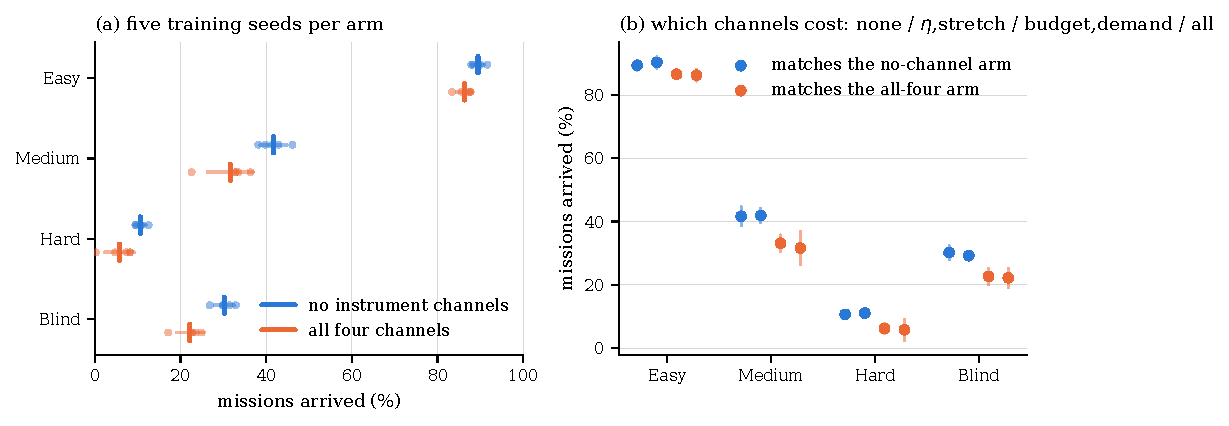
\includegraphics[width=\textwidth]{figures/ablation.pdf}
\caption{(a) Final success for every training seed, no channels against all
four; dots are seeds, bars one standard deviation, the heavy tick the mean.
(b) The four-way split; in every suite the no-channel and $\eta$,stretch
arms coincide, and the $A$,$\dd$ and all-four arms coincide below them.}
\label{fig:ablation}
\end{figure}

In this environment, at this network size and step budget, appending
features that are algebraic combinations of what the observation already
contains measurably degrades a policy, while appending features that carry
physics not otherwise available does not, and there is no evidence that the
informative channels help ($\eta$ and the stretching rate are nominally
above the no-channel arm on three suites and below it on one, none
significantly). The mechanism of the cost is not isolated. Four extra input
dimensions against 285,322 parameters is a capacity account, a ratio with a
division in it is heavy-tailed even after log compression, which is a
conditioning account, and the two predict different behavior under scale
\MEASURE{training at embedding widths 256 and 384, which would separate the
two accounts}; what can be said is that an observation channel's value to a
learner depends on whether it is new rather than on whether it is true,
which is consistent with the view that a policy is a compression of its
inputs and that a channel which does not change the policy costs capacity
without buying anything \cite{lai2024,kaelbling1998}.

\subsection{Per-instance variation}
\label{sec:ghosts}

A suite success rate is one number per checkpoint, computed from a greedy
policy that takes its most probable action, and it conceals both the
policy's own stochasticity and the variation between individual task
instances, which in procedurally generated environments is known to be large
\cite{cobbe2019,kirk2023,agarwal2021}. Figure~\ref{fig:ghosts} makes both
visible by flying every saved checkpoint of one training run on one fixed
instance sixteen times with actions sampled rather than maximized
($31 \times 16 = 496$ trajectories per instance), colored by the training
update at which each attempt was flown. Early policies spray across the
field and late policies converge into bundles, which are not always the
right ones; on the hard-suite instance shown, the trained policy converges
onto a tight shuttle between its first two targets and never reaches the
third, in 0 of 496 attempts. Firstly, sampled success is far below greedy
success (the easy-suite instance shown arrives 52\% of the time when sampled
against 89\% for the greedy policy on that suite), so that the headline
number describes a behavior the policy exhibits only with its stochasticity
removed. Secondly, the spread between instances within a suite (60\%, 52\%,
8\% and 0\% on the four shown) is larger than any effect measured between
training configurations in this paper, since the channel effect of
Section~\ref{sec:instruments} is seven to ten points and two instances drawn
from the same suite differ by fifty. Thus, any claim about this environment
that rests on a handful of instances is fragile by construction (compare
Section~\ref{sec:solvable}).

\begin{figure}[p]
\centering
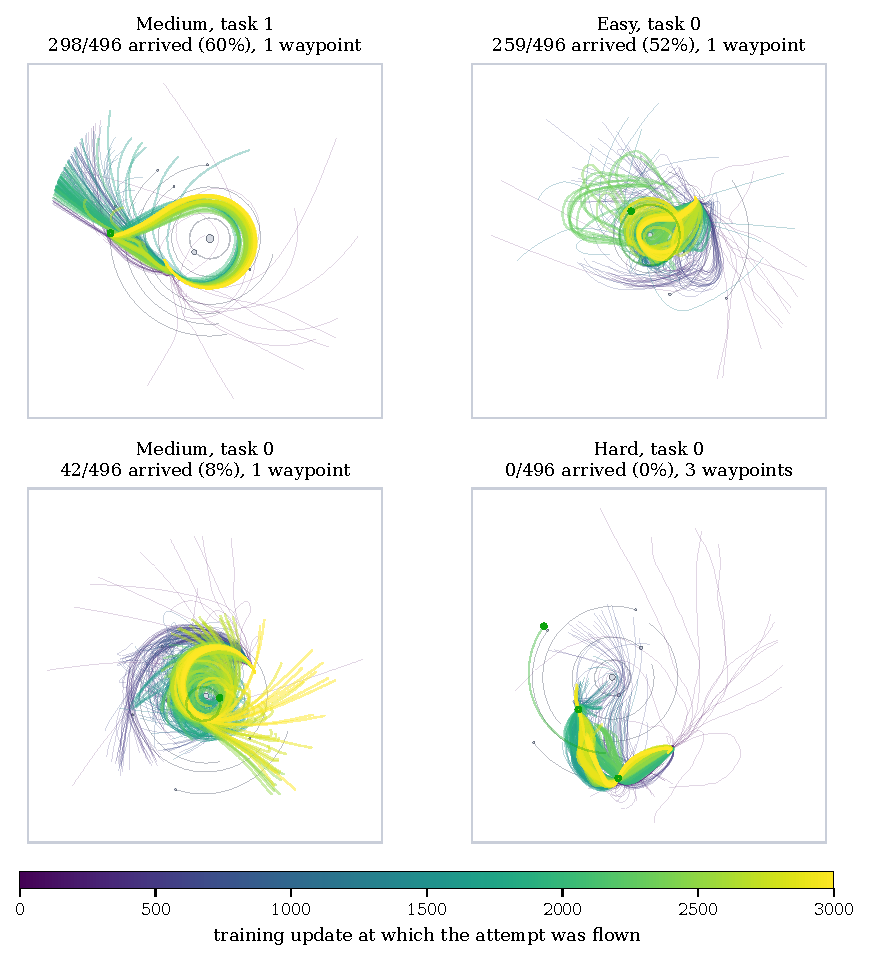
\includegraphics[width=\textwidth]{figures/ghosts.pdf}
\caption{Four task instances from the evaluation suites, each flown 496
times by one training run (every saved checkpoint, sixteen sampled rollouts
each), colored by the training update at which the attempt was flown. Grey
discs are bodies with their orbits traced faintly; green rings are targets,
drawn along their own paths where attached to moving bodies. Early policies
(dark) spray across the field; late policies (bright) converge into bundles.
Medium task 1 converges onto a single arrival corridor; medium task 0 onto
a corridor that mostly misses; hard task 0 onto a shuttle between its first
two targets that never reaches the third, at upper left.}
\label{fig:ghosts}
\end{figure}

Figure~\ref{fig:curves} gives the corresponding learning curves, which show
that mid-run checkpoints are noisy enough that the difference between two
configurations read at a third of the way through training can have the
opposite sign from the difference at the end.

\begin{figure}[t]
\centering
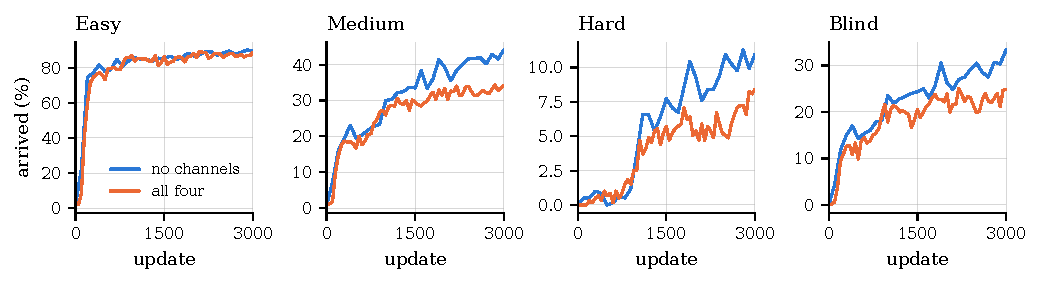
\includegraphics[width=\textwidth]{figures/curves.pdf}
\caption{Suite success against training update for one seed of each
headline configuration.}
\label{fig:curves}
\end{figure}

\subsection{Relations between the measures}
\label{sec:correlations}

The quantities of Section~\ref{sec:heuristics} were defined to describe a
level's difficulty before anyone flies it, and the test of that is whether
they predict who arrives. Across the 2,388 task instances of the four 150\,s
suites, with agent success per instance taken as the fraction of four
3000-update policies (two no-channel seeds and two all-channel seeds) that
arrived at their final checkpoint, success falls monotonically with $\dd$
(Figure~\ref{fig:corr}(a); Spearman $\rho = -0.585$, $p = 10^{-219}$), from
84\% in the lowest decile to 0.2\% in the highest, with a plateau over
$\dd \approx 0.003$--$0.05$ and a cliff above $\dd \approx 0.2$, and the
reference pilot follows the same curve ($\rho = -0.547$; the two navigators'
per-instance successes correlate at $\rho = 0.787$). A logistic model of
agent success on family alone reaches a held-out area under the curve of
$0.745$; $\dd$ alone reaches $0.811$ and family with $\dd$ reaches $0.871$,
and adding $\dd$ to a model that already knows the suite, the family, the
number of targets and whether a rendezvous is required still drops the
held-out deviance by 1042 on one degree of freedom ($p = 10^{-228}$;
ten-fold cross-validation repeated five times). Thus, $\dd$ predicts success
better than family alone and better than the suite's own design levers, as
it was meant to.

However, it does so for the wrong half of itself. Separating the ratio into
its parts, the authority $A$ alone is the stronger predictor ($\rho = +0.754$;
held-out area $0.946$ with the design levers), while $\eta$ at the targets is
weak ($\rho = -0.248$) and, once $A$ is in the model, carries no information
at all (deviance drop $0.2$ on one degree of freedom, $p = 0.67$; coefficient
$-0.02$ against $+2.09$ for $A$). The relation between success and $\eta$ is
in fact non-monotone (Figure~\ref{fig:corr}(b)): it peaks near
$\eta \approx 0.005$ and falls on both sides, and the low-$\eta$ failures
are the hazard families (\code{debris\_maze} 25\%, \code{asteroid\_field}
28\%, \code{compact\_system} 31\%, \code{pulsar} 39\%), where the field is
simple and the route is not. What the learned policy's success tracks at
this training budget is the tank against the tour, i.e. whether a direct
flight is affordable, and not whether a one-body representation of the field
is wrong; the representational component of difficulty that the dial was
built to capture is not yet the component that limits the learner. This is
consistent with the budget result of Section~\ref{sec:budget}, in which the
policy is still improving rapidly at 3000 updates, since a policy that has
not yet learned to spend its tank well fails on fuel before it can fail on
representation, and whether $\eta$ becomes predictive once $A$ is no longer
the limit is a question the 10,000-update policies could answer and the
present ones cannot. At the level of families (Figure~\ref{fig:corr}(c)) the
picture is the same from the other side: a family's median $\dd$ predicts its
success rate ($\rho = -0.734$ over the twelve families, $p = 0.007$), and the
families that break the ordering are the ones whose difficulty is hazard
rather than field.

The expectation that a longer clock matters most on multi-target tasks does
not survive normalization. On the 600\,s suites, a coasting craft first
contacts a target after the 150\,s mark on 2.3\% of single-target and 4.7\%
of multi-target tasks (Fisher's exact $p = 0.001$), but per target slot the
rates are 2.3\% and 2.1\% ($p = 0.81$), and for the first target alone 2.3\%
and 2.2\%; more targets are more chances, and the tour structure adds
nothing. Note that this measurement is on different levels from the 150\,s
suites and is not joined to the agent's per-instance success.

\begin{figure}[t]
\centering
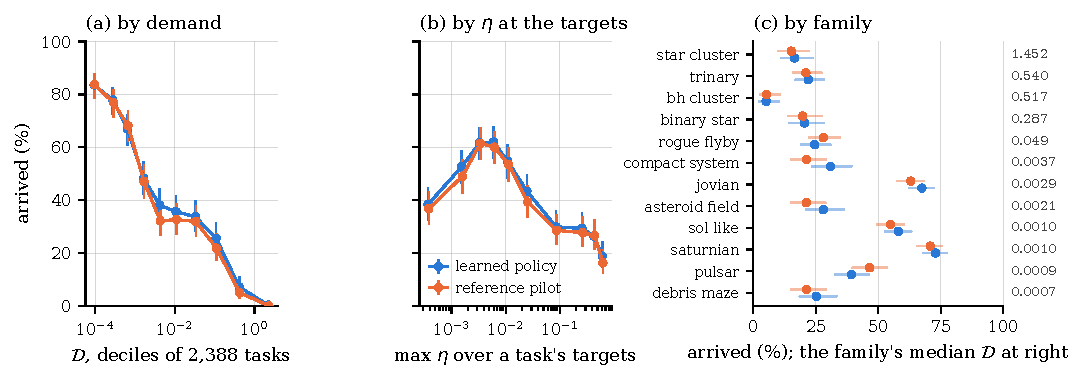
\includegraphics[width=\textwidth]{figures/corr.pdf}
\caption{Per-instance success of the learned policy (mean of four 3000-update
runs) and of the reference pilot across the 2,388 tasks of the 150\,s
suites. (a) By decile of $\dd$, with 95\% Wilson intervals. (b) By the
maximum $\eta$ over a task's targets; the relation is non-monotone, and the
low-$\eta$ failures are the hazard families. (c) By family, with each
family's median $\dd$ at right. Computed by \code{scripts/correlations.py}.}
\label{fig:corr}
\end{figure}

% =====================================================================
\section{Discussion}
\label{sec:discussion}

Although the task examined here is fully specified and cheap to simulate, it
does not admit a one-dimensional notion of difficulty, which is the first
thing this paper is meant to establish and the reason the second and third
pictures of Section~\ref{sec:framings} exist alongside the first. A learner
that treats the task as an undifferentiated observe-act-reward loop will
learn it on levels where a coarse representation suffices and will have no
particular reason to do better on levels where it does not, and the results
of Section~\ref{sec:results} are consistent with that account, the policy
being strong on the hierarchical families, weak on the contested ones and
worst on the held-out families where the representation learned elsewhere
does not transfer.

\subsection{Learning a class of levels}

The pedagogical question that follows is how an agent should be brought up
the stack of strategies in Section~\ref{sec:framings} so that what it learns
on one level is the representation it needs on the next rather than a policy
fitted to that level's particular geometry, which is the question the
literature on generalization across procedurally generated levels and on
learning to learn across task distributions addresses from two directions
\cite{cobbe2019,kirk2023,finn2017,duan2016,beck2025}. The curriculum used
here (rendezvous share, tour length, contested share, each ramped over
training) is a crude version of this, since the contested share was held at
zero until the agent could fly at all, which is to say that the agent
learned a one-body representation first and was then asked to extend it,
and whether that order helps or hinders is a question the present data
cannot answer. The literature on choosing which instances to train on next
\cite{portelas2020,florensa2018,matiisen2020,dennis2020,jiang2021,jiang2021a,parkerholder2022,jiang2022}
offers tools, with the caveat that several of its curriculum signals
correlate with an agent's success rate rather than with its regret, and so
miss the instances an agent can sometimes solve but not reliably
\cite{rutherford2024}, which are the instances the stack of strategies says
are the informative ones. What the closed-form $\dd$ offers to this problem
is a curriculum axis that a generator can set directly, placing an instance
at a chosen share-of-tank cost of a wrong representation, so that an agent
can be walked up that axis instead of being shown harder levels in the hope
that they are hard in the right way.

\subsection{Learning over a chaotic simulation}

The second picture asks for something the first cannot provide, which is a
policy that bounds its exit from a region it cannot plan through. The
measurement in Section~\ref{sec:chaos} says that the present environment
does not yet contain such regions on episode timescales, which limits the
environment and not the picture, and the route to building them is known
(Section~\ref{sec:chaos}). Once they exist, and since
the H\"older result says a policy gradient cannot be computed usefully
inside such a region, the relevant question is whether a policy can learn
the bounding behavior at the region's entrance and the adaptive behavior at
its exit while treating the interior as noise, which is closer to the robust
and tube-based formulations of control \cite{mayne2005,mitchell2005} than to
anything in standard reinforcement learning, and closer still to the
observation from flow control that the gradient through a chaotic system is
correct and useless at once \cite{metz2021,parmas2018,suh2022}. Whether the
learned representation survives passage through such a region is the
question that would decide between a model-free and a model-based approach,
and the present data do not reach it.

\subsection{Choices in the definitions}

Several of the definitions in this paper are choices, and the reader should
know which. Firstly, the equal-pull surface is the right scale for an
episode shorter than an orbit and the wrong one for a longer episode, where
resonance overlap reasserts itself (Section~\ref{sec:eta}). Secondly, the
150\,s clock was inherited from an early version of the game and never
derived from the task, and Section~\ref{sec:clock} argues it is too short. Thirdly, the banding of trivial difficulty against
human motor limits is a reasonable scale for a game and an arbitrary one for
any other purpose. Fourthly, the reference optimizer is one configuration of
one method, and every solvability label is relative to it. Finally, the
twelve families were chosen to span the regimes the authors could think of,
with no taxonomy of the field behind them. These choices do not make the
measurements wrong; they mean that the paper offers definitions that make a
set of intuitions checkable, not a theory of difficulty for this task, which
is also the condition of the task-difficulty measures and curricula in the
literature, where the measure chosen changes what the curriculum does
\cite{furuta2021,narvekar2020,rutherford2024}. The value of better
definitions here is that they let the environment and the agents that run
over it be understood together, with the same quantities describing what a
level demands and what a learner has managed, and that is a more useful
thing to have than either description alone.

% =====================================================================
\section{Future directions}
\label{sec:future}

The most immediate extensions are the ones the measurements call for, which
are a longer clock, levels with constructed chaotic regions
(Section~\ref{sec:chaos}), and training budgets and seed counts large enough
that the scaling behavior of the observation-channel result can be read.
Beyond navigation itself, the same field and the same representational
questions arise in adversarial situations, such as in a video game in which
one craft may be attempting to catch, target, or otherwise react to another,
where the moving target is itself a navigator
\cite{mitchell2005,reif1994,dennis2020}.

\section*{Acknowledgements}

The environment, the experiments and the analysis reported here were
developed in collaboration with Claude (Anthropic), operating as an
autonomous agent with access to the repository and compute; the
repository's decision records were written during that process.

% =====================================================================
\appendix
% Appendix A. Fragment, \input by spacenav.tex inside \appendix.
% Every count below was measured by running observe() on task 0 of the frozen
% medium suite (data/eval/suites.pkl, level 0 of val_seen) at reset:
%   self (109,)  bodies (32, 24)  body_mask (32,)  zones (12, 15)  zone_mask (12,)
% Formulas are transcribed from spacenav/env.py observe() and instrument_panel().

\section{The observation vector}
\label{app:obs}

What the policy is given at each control tick is the output of
\code{observe()} in \code{spacenav/env.py}, a dictionary of fixed-shape arrays
rather than a single vector, so that a level with seven bodies and one with
thirty-two produce the same shapes and can share a batch: a self block of 109
numbers; one token of 24 numbers for each of the 32 body slots, with a 32-entry
mask marking which slots hold a body; and one token of 15 numbers for each of
the 12 hazard-zone slots, with a 12-entry mask, which is 1,057 numbers in all
(109 + 32 $\times$ 24 + 12 $\times$ 15, as measured by running \code{observe()}
on a task from the frozen medium suite). Everything is expressed in the craft's
own frame, i.e. positions and velocities are taken relative to the craft and
rotated so that its nose lies along $+x$, with two fixed scales, $L = 100$\,u
for lengths and $V = 20$\,u/s for speeds, and a signed logarithmic compression
$\mathrm{symlog}(x) = \mathrm{sign}(x)\ln(1 + |x|)$ applied wherever a quantity
spans several orders of magnitude. Throughout the tables, $a_{\mathrm{eng}}$ is
the task's engine acceleration, $a_{\max} = 4$\,u/s$^2$ is the fixed upper end
of the engine range (\code{SHIP\_ACCEL}, used only as a normalizer), $R$ is the
level radius, $T_{\max}$ is the episode clock (150\,s unless
\code{SPACENAV\_EPISODE\_S} says otherwise, Appendix~\ref{app:repro}), and
``the target'' is the waypoint currently being flown to, which in a fixed-order
tour is the next unvisited one and in an order-free tour is the nearest
unvisited one (Appendix~\ref{app:goals}).

\begin{table}[htbp]
\centering
\footnotesize
\begin{tabular}{p{4.3cm}p{6.6cm}r}
\toprule
Entry & Formula or source & Dim.\ \\
\midrule
\multicolumn{3}{l}{Craft and field} \\
craft velocity & $\mathrm{rot}(v)/V$ & 2 \\
local gravity & $\mathrm{rot}(g)/a_{\max}$, $g$ the full field at the craft & 2 \\
\multicolumn{3}{l}{The target} \\
relative position & $\mathrm{symlog}(\mathrm{rot}(x_t - x)/L)$ & 2 \\
bearing & unit vector of $\mathrm{rot}(x_t - x)$ & 2 \\
distance & $\mathrm{symlog}(\lVert x_t - x\rVert/L)$ & 1 \\
relative velocity & $\mathrm{rot}(v_t - v)/V$ & 2 \\
\multicolumn{3}{l}{Loadout, tour and state} \\
fuel fraction & $\mathrm{fuel}/\mathrm{fuel}_0$, seconds of burn left over seconds carried & 1 \\
$\Delta v$ remaining & $\mathrm{fuel}\cdot a_{\mathrm{eng}}/100$ & 1 \\
$\Delta v$ remaining over required & $\mathrm{fuel}\cdot a_{\mathrm{eng}} / (\Delta v_{\mathrm{req}} + 10^{-3})$ & 1 \\
$\Delta v$ required & $\mathrm{symlog}(\Delta v_{\mathrm{req}}/100)$, from \code{deltav\_estimate} over the pending legs & 1 \\
engine & $a_{\mathrm{eng}}/a_{\max}$ & 1 \\
health & health$/100$ & 1 \\
time remaining & $1 - t/T_{\max}$ & 1 \\
pending targets & number unvisited $/\,6$ & 1 \\
order-free flag & 0 or 1 & 1 \\
damage rate & $\mathrm{symlog}$ of the current damage rate (health/s) & 1 \\
exposure & soft-edged membership, 0--1, of the zone the exposure objective charges for & 1 \\
radial position & $\lVert x\rVert/R$ & 1 \\
objective weights & time, path, fuel, exposure; sum to one & 4 \\
instrument panel & $\eta$, $\mathrm{symlog}\,A$, $\mathrm{symlog}\,\dd$, $10\times$stretch, each times its 0/1 mask & 4 \\
\multicolumn{3}{l}{Per waypoint slot, six slots, 13 each} \\
relative position & $\mathrm{symlog}(\mathrm{rot}(x_k - x)/L)$ & 2 \\
bearing & unit vector of $\mathrm{rot}(x_k - x)$ & 2 \\
distance & $\mathrm{symlog}(\lVert x_k - x\rVert/L)$ & 1 \\
relative velocity & $\mathrm{rot}(v_k - v)/V$ & 2 \\
arrival radius & $r_k/L$ (always $0.12$) & 1 \\
velocity tolerance & $\min(v^{\mathrm{tol}}_k, 50)/V$ ($0.15$ for a rendezvous, $2.5$ for a flythrough) & 1 \\
four flags & visited; is the current target; active; anchored to a body (0/1 each) & 4 \\
\midrule
total & $31 + 6 \times 13$ & 109 \\
\bottomrule
\end{tabular}
\caption{The self block. $x$, $v$ are the craft's position and velocity, $x_t$,
$v_t$ the current target's, $x_k$, $v_k$ the $k$-th waypoint slot's (an
inactive slot reports the position its sampler left in it, masked by the
active flag), and $\mathrm{rot}$ the rotation into the craft's frame.}
\label{tab:obs-self}
\end{table}

\begin{table}[htbp]
\centering
\footnotesize
\begin{tabular}{p{4.3cm}p{6.6cm}r}
\toprule
Entry & Formula or source & Dim.\ \\
\midrule
relative position & $\mathrm{symlog}(\mathrm{rot}(x_b - x)/L)$ & 2 \\
bearing & unit vector of $\mathrm{rot}(x_b - x)$ & 2 \\
distance & $\mathrm{symlog}(d/L)$, $d = \lVert x_b - x\rVert$ & 1 \\
relative velocity & $\mathrm{rot}(v_b - v)/V$ & 2 \\
pull & $\mathrm{symlog}\big(GM_b / \max(d, r_b)^2 / a_{\mathrm{eng}}\big)$, the body's acceleration on the craft in units of the engine & 1 \\
mass & $\ln(1 + GM_b)/10$ & 1 \\
radius & $r_b/L$ & 1 \\
atmosphere & thickness$/L$ (0 for none) & 1 \\
luminosity & $\ln(1 + \mathrm{lum}_b)/10$ & 1 \\
clearance & $(d - r_b - \text{thickness})/L$, signed & 1 \\
carries a target & 1 if any active waypoint is anchored to this body & 1 \\
kind & one-hot over ten kinds (none, star, rocky, giant, moon, black hole, station, asteroid, tracer, neutron star) & 10 \\
\midrule
total & & 24 \\
\bottomrule
\end{tabular}
\caption{The body token, one per slot for 32 slots, with the mask
\code{body\_mask} equal to the level's \code{active} flags. $x_b$, $v_b$, $GM_b$
and $r_b$ are the body's position, velocity, gravitational parameter and
radius. Stations and tracers are massless and have zero pull; a tracer is the
invisible anchor of a moving zone.}
\label{tab:obs-body}
\end{table}

\begin{table}[htbp]
\centering
\footnotesize
\begin{tabular}{p{4.3cm}p{6.6cm}r}
\toprule
Entry & Formula or source & Dim.\ \\
\midrule
relative position of the center & $\mathrm{symlog}(\mathrm{rot}(x_z - x)/L)$, $x_z$ the anchor body's position (the origin for an unanchored zone) & 2 \\
bearing & unit vector of $\mathrm{rot}(x_z - x)$ & 2 \\
distance to the center & $\mathrm{symlog}(d_z/L)$ & 1 \\
inner radius & $r_{\mathrm{in}}/L$ & 1 \\
outer radius & $r_{\mathrm{out}}/L$ & 1 \\
signed distance to the band & $\mathrm{symlog}\big(\max(r_{\mathrm{in}} - d_z,\; d_z - r_{\mathrm{out}})/L\big)$, negative inside & 1 \\
kind & one-hot over none, debris, radiation, sensor & 4 \\
strength & the zone's damage coefficient & 1 \\
spin & $+1$/$-1$ if the debris circulates around the anchor, 0 if it moves with it & 1 \\
counts as exposure & 1 if this is the zone the task's exposure objective charges for & 1 \\
\midrule
total & & 15 \\
\bottomrule
\end{tabular}
\caption{The zone token, one per slot for 12 slots, with the mask
\code{zone\_mask} equal to the level's \code{zone\_active} flags. A zone is an
annulus between $r_{\mathrm{in}}$ and $r_{\mathrm{out}}$ around its anchor,
with a soft edge of 15\% of its thickness.}
\label{tab:obs-zone}
\end{table}

The four instrument channels occupy the last four entries of the self block
before the waypoint slots, in the order $\eta$, $A$, $\dd$, stretch, and are
computed by \code{instrument\_panel()} at the craft's position from the same
quantities the body of the paper defines: $\eta$ is
$\lVert g_{\mathrm{full}} - g_{\mathrm{dom}}\rVert / \lVert g_{\mathrm{full}}\rVert$
with $g_{\mathrm{dom}}$ the field restricted to the single strongest attractor
(\code{gravity\_at(topk=1)}); the authority $A$ is
$\mathrm{fuel}\cdot a_{\mathrm{eng}} / (\lVert g_{\mathrm{full}}\rVert\,T_{\mathrm{left}})$
with $T_{\mathrm{left}}$ the time to the clock, floored at one control tick,
and is passed through symlog; the demand $\dd = \eta/A$ is likewise passed
through symlog; and the stretching rate is
$\sqrt{\sum_b 2\,GM_b / r_b^3}$ over the active bodies, i.e. the square root
of the summed tidal gradient (a rate in 1/s, with $r_b$ floored at the body's
radius or 1\,u), multiplied by ten so that it sits in the same range as the
other entries. Each channel is then multiplied by a 0 or 1 taken from the
environment variable \code{SPACENAV\_INSTRUMENTS}, which is read once when
\code{spacenav.env} is imported and accepts, in order of specificity, \code{0}
(or \code{off}, or the empty string) to zero all four, \code{1} (or \code{on},
\code{all}) to pass all four, a comma-separated subset of the names
\code{eta}, \code{budget}, \code{demand}, \code{stretch} (the names the code
gives $\eta$, $A$, $\dd$ and the stretching rate; an unknown name raises), or a
four-character mask of 0s and 1s in that order, with \code{eta,stretch} as the
default (the \code{eta,stretch} arm of Table~\ref{tab:instr}; the no-channel
arm is \code{0} and the all-four arm \code{1}). Because a zeroed channel keeps
its slot, the observation shape, and hence the network, is identical under
every setting, and nothing checks that a checkpoint is evaluated under the
setting it was trained under; a policy trained with a channel live and
evaluated with it zeroed reads a zero where it learned to expect a value, and
the converse reads a value where it learned to expect a zero, in both cases
without an error and with a success rate that simply looks wrong. The setting
a run was trained with is written to its \code{config.json} under
\code{instruments}, and \code{SPACENAV\_INSTRUMENTS} should be set to that
string whenever the run's checkpoints are replayed or evaluated.

The body and zone tokens are each passed through a two-layer embedding to a
width of 128 and concatenated into one set of 44 tokens, which the network
pools in two ways at once, by multi-head cross-attention (four heads) in which
the embedded self block is the query and the tokens are keys and values, with
the masked slots given an attention logit of $-10^9$ so that they receive no
weight, and by an element-wise maximum over the unmasked tokens' rectified
embeddings; the self embedding and the two pooled summaries are concatenated
and fed to the shared policy and value trunk. Neither pooling depends on the
number of bodies or on their order in the slots, which is what allows the same
weights to run on every level, and it is why a level's bodies can be stored
and presented in whatever order its generator produced them.


\section{Theoretical notes on observation}
\label{app:theory}

The observation of Appendix~\ref{app:obs} is exact and instantaneous: at
every control tick the policy is handed the true position and velocity of
every body and target as of that tick. Two departures from this are worth
setting down, because each would change what a learner could and could not
infer, and because the environment's construction makes one of them
unusually clean to study.

The first is a finite signal speed. If the craft learned of a body's state
by light, a body at distance $r$ would be seen where it was a time $r/c$
ago, and at game scale this is not negligible: with a signal speed chosen so
that the far side of a 3000\,u level is one control tick away ($c \approx
45{,}000$\,u/s, or one level-crossing per 66.7\,ms), a body at 300\,u would
be seen one tenth of a tick late and a body across the level a full tick
late, so that the observation would be internally inconsistent, with near
bodies reported more recently than far ones. A learner given such an
observation faces a problem that the present one does not pose, which is
that the state it is handed is not the state of any single instant, and the
correction (extrapolating each body forward by its own delay) requires the
body's velocity, which is itself delayed. Whether a policy of the size used
here can learn that correction implicitly, and at what cost in success, is
an experiment the environment supports with a change to \code{observe()}
alone, since the delayed state is available from the stored ephemeris; it
has not been run. The formal setting for it is the partially observable
Markov decision process \cite{kaelbling1998}, in which the delayed
observation defines a belief over the current state.

The second is the distinction between a projected observation and a
measured one, and here the environment's design has a consequence that is
easy to overlook. Because the craft is a test particle, the bodies' future
is fixed by the level's initial snapshot, and a navigator that knows the
snapshot can compute every body's position at every future tick exactly,
which is what the browser client does when it integrates the ephemeris
itself from 1.5\,KB of state. The observation the policy receives is
therefore equivalent to a projection from the snapshot, and nothing in it
is a measurement in the sense of a quantity that could have come out
otherwise. In a real setting the two differ: a measured position carries
sensor noise, a projected one carries model error that grows with the
projection horizon, and a navigator must weigh one against the other. The
present environment collapses the distinction by construction, which is a
simplification to be aware of when reading the results, and which the
instrument channels of Section~\ref{sec:instruments} partly reintroduce,
since $\eta$ is exactly a measure of how wrong a one-body projection of the
field would be. A version of the task in which the craft perturbs the bodies
(so that the ephemeris cannot be precomputed) or in which body positions
are observed with noise (so that projection and measurement disagree) would
restore the distinction, and the second is cheap to add.

% Appendix C. Fragment, \input by spacenav.tex inside \appendix.
% Transcribed from spacenav/env.py: _sample_waypoint, sample_tour, current_leg,
% waypoint_states, deltav_estimate, _substep, step; spacenav/physics.py
% hazard_terms; spacenav/constants.py.

\section{Goal conditions}
\label{app:goals}

A task instance is a tour of between one and six waypoints, sampled one after
another by \code{sample\_tour()} in \code{spacenav/env.py} so that each lies at
least 100\,u (\code{min\_leg}) from the one before it, and each is of one of
the three kinds in Table~\ref{tab:goal-kinds}, which differ in what the
waypoint is attached to and therefore in how it moves. Whether a waypoint
moves is decided first (with probability \code{p\_station}, 0.35 by default
and set per suite), and a moving waypoint is a station when the level has a
free one and a coin comes up heads, otherwise a point hung off a solid body; a
waypoint that does not move is a point sampled uniformly over the playable
disc, rejected and redrawn (up to 96 candidates) until it lies between
\code{min\_dist} and \code{max\_dist} from the previous waypoint, inside 0.9 of
the level radius, at least 20\,u clear of every surface and atmosphere, and at
a point where the instantaneous damage rate is under 0.3 health/s. The
velocity condition is drawn second and only for a moving waypoint, with
probability \code{p\_rendezvous} (so that the rendezvous shares quoted in
Table~\ref{tab:suites} are conditional on the waypoint moving, and a fixed
point in free space is always a flythrough). Every waypoint has the same
arrival radius of 12\,u (\code{TARGET\_RADIUS}), and the craft is at a waypoint
when, at the end of a physics substep, both its distance to the waypoint's
current position is under 12\,u and its speed relative to the waypoint's
current velocity is under the waypoint's tolerance, which is 3\,u/s
(\code{RENDEZVOUS\_V\_TOL}) for a rendezvous and $10^9$\,u/s, i.e. any speed,
for a flythrough. Both conditions are evaluated against the waypoint's state
at that substep, so a rendezvous with a station is a velocity match with the
station's orbital motion and a rendezvous with a point hung off a giant is a
match with the giant's.

\begin{table}[htbp]
\centering
\footnotesize
\begin{tabular}{p{2.5cm}p{4.6cm}p{2.7cm}p{2.9cm}}
\toprule
Kind & Where it is & How it moves & Velocity condition \\
\midrule
\raggedright free-space point & \raggedright a fixed position in the level frame, sampled as above (\code{wp\_anchor} $= -1$) & \raggedright it does not; its velocity is zero & \raggedright flythrough only \tabularnewline
\raggedright station & \raggedright the position of a station body (massless, zero radius, on its own orbit around its host) & \raggedright with the station & \raggedright flythrough or rendezvous with the station's velocity \tabularnewline
\raggedright attached to a body & \raggedright the body's position plus a constant offset vector of length (radius + atmosphere + 35\,u) at a random angle, or, for a contested waypoint, of length $0.8$--$1.3\times$ the body's equal-pull radius (Section~\ref{sec:eta}) & \raggedright the offset translates with the body and does not rotate with it & \raggedright flythrough or rendezvous with the body's velocity \tabularnewline
\bottomrule
\end{tabular}
\caption{The three waypoint kinds. Every kind has the same 12\,u arrival
radius; black holes and tracers are never anchors, and a body that already
carries a waypoint is not chosen again in the same tour. The figure of the
task (Figure~\ref{fig:task}d) shows the same conditions as four cells by
separating the velocity condition from the attachment.}
\label{tab:goal-kinds}
\end{table}

A tour is flown in slot order unless the instance's \code{order\_free} flag is
set (with probability \code{p\_order\_free}, zero in training until the
curriculum raises it and 0.3 on the blind suite), and the difference between
the two is only in which waypoint an arrival is credited to: in a fixed-order
tour, reaching a waypoint counts only if it is the next unvisited one in slot
order, so that passing through the third waypoint on the way to the first does
nothing, while in an order-free tour any unvisited waypoint counts whenever its
conditions are met. The observation's notion of the current target
(Appendix~\ref{app:obs}) follows the same rule, being the next unvisited
waypoint in a fixed-order tour and the nearest unvisited one in an order-free
tour, and so does the potential used for reward shaping, which is the negative
of the distance to the current target plus a flat allowance for each further
waypoint still outstanding. The scoring of a completed tour is identical in
the two cases (the same per-waypoint and completion rewards, the same weighted
cost over time, path, fuel and exposure), so an order-free tour is neither
easier nor harder by construction; it is different in that the navigator, and
not the instance, chooses the sequence.

The craft's loadout is drawn against the tour it has to fly. With $d_k$ the
straight-line length of the $k$-th leg (from the start position to the first
waypoint and then from each waypoint to the next, in slot order and ignoring
gravity, the craft's initial velocity and any motion of the waypoints), the
$\Delta v$ the tour is estimated to require is
\begin{equation}
\Delta v_{\mathrm{req}} \;=\; \sum_k
\begin{cases}
\sqrt{2\,a_{\mathrm{eng}}\,d_k} & \text{flythrough, i.e. accelerate across the whole leg,}\\[2pt]
2\sqrt{a_{\mathrm{eng}}\,d_k} & \text{rendezvous, i.e. accelerate for half the leg and brake for half,}
\end{cases}
\end{equation}
which \code{deltav\_estimate()} computes and which is also what the
observation reports as the $\Delta v$ required over the legs still pending.
The engine acceleration $a_{\mathrm{eng}}$ is drawn log-uniformly from
$[0.6, 3]$\,u/s$^2$ (\code{SHIP\_ACCEL\_RANGE}, narrowed to $[1.5, 3]$ on the
easy suite and $[0.8, 2]$ on the hard suite, and started generous by the
training curriculum), the budget multiple $\beta$ is drawn uniformly from
$[0.55, 1.35]$ (\code{DELTAV\_BUDGET\_RANGE}, narrowed per suite as
Table~\ref{tab:suites} lists), and the tank, in seconds of full-throttle burn,
is $\beta\,\Delta v_{\mathrm{req}} / a_{\mathrm{eng}}$ clipped to
$[3, 60]$\,s (\code{SHIP\_FUEL\_LIMITS}), so that the tank actually carried can
be a larger multiple of the estimate than $\beta$ on a very short tour and a
smaller one on a very long tour. The reference scales that normalize the four
cost terms are set from the same quantities, with the time and exposure
references equal to $\sum_k 2\sqrt{d_k/a_{\mathrm{eng}}}$, the path reference
equal to $\sum_k d_k$ and the fuel reference equal to half the tank, and the
objective weights are either a single objective (with probability 0.5, drawn
with probabilities 0.4, 0.2, 0.3 and 0.1 over time, path, fuel and exposure)
or a Dirichlet mixture of them, with exposure available only on a level that
has at least one zone, the zone charged for being drawn from the level's
active zones with sensor zones favored by a factor of $e$ over the rest.

An episode ends in exactly one of five ways, tested in this order at the end
of every physics substep (60\,Hz) and reported as the status code the
evaluation suites count: \code{crashed}, the craft's position is inside the
radius of a solid body (a station or a tracer, having no radius, cannot be
crashed into); \code{destroyed}, health has reached zero under the accumulated
damage from stellar radiation, atmospheric heating, debris and radiation
belts; \code{arrived}, every active waypoint has been visited, which is the
only success; \code{lost}, the craft is farther than 1.35 times the level
radius from the origin; and, tested once per control tick rather than per
substep, \code{timeout}, the tick count has reached $T_{\max}/\Delta t$ (2250
at the 150\,s clock) with the tour unfinished. An empty tank is not among
them. The burn in a substep is the smaller of the commanded burn and the fuel
left, so that once the tank is empty the throttle does nothing, the craft
coasts under gravity alone, and the episode continues until one of the five
endings occurs, which on an energy-efficient path is often the clock
(Section~\ref{sec:clock}) and on a decaying one is a crash. The hazard terms
themselves do not end an episode; they lower health, and only health reaching
zero does.


% Appendix D. Fragment, \input by spacenav.tex inside \appendix.
% Commands transcribed from the scripts' own usage lines; versions from
% requirements-gpu.txt and the conda environment the runs were made in.

\section{Reproduction}
\label{app:repro}

Everything reported in this paper is produced by scripts in the repository,
from a checkout with the \code{spacenav} package installed and the GPU build
of JAX, in the order below; \code{data/} is not under version control, and the
level pools are regenerated from their seed blocks (seeds from 0 for the
training pool, from $10^7$ for the seen-family validation pool, from
$2 \times 10^7$ for the holdout pool, from $3 \times 10^7$, $4 \times 10^7$
and $5 \times 10^7$ for the three long-horizon pools: \code{long}, the
\code{long\_val} pool the 600\,s suites are drawn from, and the 900-level pool
validated to 9{,}000\,s) so that the levels themselves
are reproducible without being distributed.

\begin{small}
\begin{verbatim}
# level pools: train, val_seen, val_holdout (data/pools/*.npz), then the
# long-horizon pool used at a 600 s clock
python scripts/build_pools.py --train 2000 --val 300 --holdout 400
SPACENAV_EPISODE_S=600 python scripts/build_pools.py --only long --n 200

# one training run at the 150 s clock; the frozen suites
# (data/eval/suites.pkl) are built on first use
SPACENAV_INSTRUMENTS=eta,stretch \
  python scripts/train.py --run abl_info_s0 --updates 3000 --seed 0 --pool train
SPACENAV_INSTRUMENTS=0 \
  python scripts/train.py --run ppo_v5_noinstr --updates 3000 --seed 0
SPACENAV_INSTRUMENTS=1 \
  python scripts/train.py --run ppo_v4 --updates 3000 --seed 0
SPACENAV_INSTRUMENTS=budget,demand \
  python scripts/train.py --run abl_redundant_s0 --updates 3000 --seed 0

# the 600 s clock: suites from the long_val pool (built here on first use),
# then training on the long pool against them
SPACENAV_EPISODE_S=600 python scripts/build_long_suites.py --clock 600
SPACENAV_EPISODE_S=600 SPACENAV_SUITES=data/eval/suites_long.pkl \
  python scripts/train.py --run long600_s0 --updates 3000 --seed 0 --pool long

# the clock sweep (the reference optimizer at 150, 300, 600 and 900 s)
bash scripts/clock_sweep.sh data/curriculum/clock

# the ghost fleets: every checkpoint of one run on one instance, rolled out
# with the instrument setting the run was trained with
SPACENAV_INSTRUMENTS=eta,stretch python scripts/ghost_fleet.py \
  --run abl_info_s0 --suite medium --task 1 --rollouts 16 \
  --out data/ghosts/medium_1.json

# the zero-thrust navigator to 900 s, the 9,000 s pool, and the same to 9,000 s
python scripts/noop_clock.py measure --clock 900
python scripts/noop_clock.py build10x --per-family 100
python scripts/noop_clock.py measure10x --clock 9000
python scripts/noop_clock.py figure

# per-instance success against eta, A, D and family
python scripts/correlations.py

# the training-budget run
SPACENAV_INSTRUMENTS=eta,stretch \
  python scripts/train.py --run budget10k_s0 --updates 10000 --seed 0

# figures
python scripts/paper_figures.py --which ghosts,ablation,clock,curves,eta
python scripts/fig_task.py --suite hard --task 63 --run ppo_v5_noinstr
python scripts/fig_phase.py compute --pool data/pools/long.npz
python scripts/fig_phase.py render
\end{verbatim}
\end{small}

Two environment variables select the process-wide settings that the body of
the paper varies. \code{SPACENAV\_EPISODE\_S} sets the episode clock in
seconds (default \code{150.0}) and is read once, at import, by
\code{spacenav/constants.py}, from which the tick count, the time-remaining
entries of the observation and the number of snapshots a pool stores are all
derived; a clock longer than the window a pool was validated over (300\,s for
\code{train} and the two validation pools, 900\,s for the long-horizon pools)
runs late-starting episodes past where the level was checked, which is why the
long clock has its own pools and its own suites, selected with
\code{SPACENAV\_SUITES}, and why \code{train.py} refuses to build a
non-default suite file on its own. \code{SPACENAV\_INSTRUMENTS} selects which
of the four instrument channels are live (Appendix~\ref{app:obs}), with the
training default \code{eta,stretch}, and since every setting produces the same
observation shape a checkpoint must be evaluated or replayed under the setting
recorded in its run's \code{config.json}, as nothing will complain if it is
not. Every evaluation reported here is the greedy policy (the most probable
action at each tick) on the frozen suites, written by \code{train.py} to
\code{eval.jsonl} at every fiftieth update, with the quoted success rate being
the mean of a run's last three checkpoints; the ghost-fleet replays are the
one place actions are sampled.

The simulation, environment, optimizer and training loop are written in
Python 3.12 against JAX 0.9.2 (the \code{jax[cuda12]} build), with the policy
network in Flax 0.12.6 and the optimizer state in Optax 0.2.8; array handling
and the statistics in the figure scripts use NumPy 2.4.3 and SciPy 1.17.1, and
the figures are drawn with matplotlib 3.11.2, all as pinned in
\code{requirements-gpu.txt} and installed in the conda environment the runs
were made in. The browser client in \code{web/} is a direct port of the
physics in JavaScript, and a parity test (\code{tests/test\_js\_parity.py})
holds the two integrators to the same trajectories, which is what makes the
replays on the companion site the flights that were scored rather than
re-renderings of them.

The twenty headline runs were made on two cards. Seeds 0 and 1 of the
no-channel and all-four arms ran on an NVIDIA GeForce GTX 1080 Ti (11\,GB,
Pascal), at about 17,000 environment steps per second averaged over a whole
run including its checkpoint evaluations (the training loop alone measures
31,900 steps/s at this network width), or 6.4\,h for 3,000 updates; the
remaining sixteen runs, and all of the long-clock runs, ran on an NVIDIA
GeForce RTX 3090 (24\,GB) at about 111,000 steps per second for a single
process, or 67\,min per run, a card that one such process already saturates,
so that two concurrent runs together deliver three quarters of the throughput
of one. Within the no-channel arm, whose seeds are split across the two cards, no
difference attributable to the card was found. The cross-entropy optimizer, the chaos probe and the phase portraits run
on either card, with the single-burn outcome maps of Figure~\ref{fig:phase}
being the one computation (368,640 full-episode rollouts per level) that is
impractical on the smaller one.

The reasoning behind every design choice, rejected approach and measurement
that changed the plan is recorded in \code{docs/decisions/}, as numbered,
append-only decision records; a reversed decision is superseded by a new
record rather than edited, so that the wrong turns remain legible, and each
record cites the script, sample size or paper that forced it. The records are
the trail from which the arguments of Sections~\ref{sec:eta}
through~\ref{sec:results} were assembled (for instance, the equal-pull surface
replacing the resonance-overlap scale, the solvability yardstick being judged
on sample size, the instrument channels being split along the redundancy
line, and the clock becoming a per-process setting), and they are the place
to look when a number in this paper and a number in the repository disagree,
since the record will say which measurement superseded which.


\bibliographystyle{unsrtnat}
\bibliography{references}

\end{document}
